\documentclass[10pt,journal,cspaper,compsoc]{IEEEtran}
\usepackage{subfigure}
\usepackage{graphicx}
\usepackage{multirow}
\usepackage{xspace}
\usepackage{color}
\usepackage{amsmath}
\usepackage[ruled, vlined]{algorithm2e}
\usepackage{amsfonts}
\usepackage{url}
\usepackage{array}  
\usepackage{booktabs}
\usepackage[nocompress]{cite}
\newcommand{\sys}{\texttt{LDA$^*$}\xspace}
\newcommand{\tabincell}[2]{\begin{tabular}{@{}#1@{}}#2\end{tabular}}
\newtheorem{theorem}{Theorem}[section]
\newtheorem{corollary}{Corollary}[theorem]
\newtheorem{lemma}[theorem]{Lemma}

% IEEEtran contains the IEEEeqnarray family of commands that can be used to

\hyphenation{op-tical net-works semi-conduc-tor}

\begin{document}

\title{TM*: A Robust and Large-scale Topic Modeling System}

% PRIOR to the title within the \IEEEtitleabstractindextext IEEEtran
% command as these need to go into the title area created by \maketitle.
% As a general rule, do not put math, special symbols or citations
% in the abstract or keywords.
\IEEEtitleabstractindextext{%
\begin{abstract}
In the last decades, Bayesian inference has been applied to many scenarios, such as information extraction, iamge understanding, probalistic databases. However, the performance of the Bayesian inference varies a lot due to the different implementations. To achieve a well-optimized one, it is not a easy task.
Our first contribution is a systematic study of all recently proposed
samplers: AliasLDA, F+LDA, LightLDA, and WarpLDA.
We discovered a novel system tradeoff
among these samplers. Each sampler has different
sampling complexity and performs differently,
sometimes by 5$\times$, on documents with different lengths.
Based on this tradeoff, we further developed a hybrid sampler
that uses different samplers for different types of documents. This
hybrid approach works across a wide range of workloads
and outperforms the fastest sampler by up to 2$\times$.
\end{abstract}


\begin{IEEEkeywords}
Topic Model, Sampling Method
\end{IEEEkeywords}}
% make the title area
\maketitle

\IEEEdisplaynontitleabstractindextext
\IEEEpeerreviewmaketitle

\IEEEraisesectionheading{\section{Introduction}\label{sec:introduction}}
\IEEEPARstart{B}{ayesian} inference and learning, a topic that has
emerged since 1980s~\cite{Pearl:1988:Book}, has become relatively
mature in recent years. The last decade has witnessed
a wide array of applications of such technique such as information extraction~\cite{zhang.thesis}, image
understanding~\cite{LeCun:2015:Nature}, probabilistic databases~\cite{Chris.book}.
However, implementing high performance
algorithms of Bayesian inference is not an
easy task, a non-optimal implementation may
by slower than well-optimized ones by one o more orders of magnitude. In this paper, we focus on
a class of Bayesian models---topic models, present a systematic
study on their inference algorithms, and introduce Liblda---an efficient, user-friendly, and easy-to-extend programming library for training and inferencing topic models.
	
Topic models are famous Bayesian models for discovering
the abstract ``topics'' that occur in a collection of
documents.
From the most famous one, topic modeling with Latent
Dirichlet Allocation (LDA), a variety of topic models have 
been proposed and spread in the last decade. Taking some typical models as examples, Supervised Topic Model (STM)
assumes that each document is attached with a response
variable so that it can take more 
information about documents into account; Topic over Time (TOT) model assumes each topic is associated with a continuous distribution over time so as to capture
how the popularity of topics changes over time; and 
Correlated Topic Model (CTM) uses the correlation matrix of Gaussian distribution to model the correlation between topics. Despite of the abundance of systems designed for 
LDA, including LightLDA, Petuum, and YahooLDA, none of 
them is designed to deal with LDA variants.
Besides, none of these systems is designed to deal with diversity and skew of workloads that we see from real-world data sets.
In this paper, we ask how to design a single system to support a variety of topic models with a diverse set of workloads. \\

\noindent
\textbf{Painpoint \& Challenge 1.}
One challenge in building such a system roots from
the diversity and skew of workloads. In our use case, users
need to run topic modeling on documents of
very different types such as web corpus, user behaviours 
logs, and social network posts.
Therefore, the length of documents varies---the average length of the NIPS dataset is about 1,000
tokens while it is only 90 for the PubMED dataset.
More significantly,  the word frequency in most 
natural language corpus follows a power law~\cite{mikolov2013distributed} distribution in which
some words are orders of magnitude more frequent
than others.
This diversity and skew of input corpus causes different
systems to slow down on different datasets we
were trying to support. Worse, there are no
studies of this tradeoff available so far.
\\

\noindent
\textbf{Painpoint \& Challenge 2.}
Another challenge in building a system to support a wide range of
topic models is the diversity of different models.
Some models are constructed with different distributions, e.g.
Dirichlet distribution in LDA and Logistic Normal distribution in CTM, while
some models support different kinds of data sets, e.g. STM
supports labeled documents and TOT supports  documents with timestamps.
To propose a general framework that can be
easily extended to inference different topic models 
with high performance, a systematic study over topic models
and their inference algorithms is needed. Although the
algorithms for LDA model have been widely studied, there 
are few studies on inference algorithms for other topic models and none
of the state-of-the-art algorithms for LDA can be applied to
inference other topic models directly.
\\

Motivated by these two challenges we faced
while trying to deploy existing systems,
we decide to build Liblda with a design that
not only integrates the recent exciting
advancement of fast inference algorithms for LDA model, but also keeps in mind the diversity and skew in datasets we saw from our industry partners.
Our approach is to systematically study a variety of
topic models and their inference algorithms, study the system tradeoff caused by the diversity and skew of the workloads, and design novel algorithms and system architectures accordingly.
As a result, Liblda can be up to 5$\times$
faster than existing systems and can be extended to
support other topic models easily.
\\

\noindent
{\bf Overview of Technical Contributions.}
We describe our technical contributions.
We first present a short summary of our study on how to apply Gibbs sampling algorithm to different topic models. 
Then we present a hybrid sampler, motivated by our systematic study of recently proposed samplers.
Finally, we introduce our {{{general algorithm framework}}}
that can be easily extended to solve different
topic models.
\\

\noindent
{\large \em Contribution 1: Topic Model Revised.}
We first focus on a systematic study over topic models
and inference algorithms. In this paper, we introduce 
four selected models, LDA, STM, TOT, and CTM, and
analyze how to apply state-of-the-art samplers of LDA to other models.

\vspace{0.5em}
{\bf (Gibbs Sampling: A Premier)}
Gibbs sampling is the {\em de facto} algorithm to solve topic modeling that has been used intensively
by previous work~\cite{harvey2013building,zhu2012medlda, yao2009efficient,li2014reducing,yu2015scalable,yuan2015lightlda, chen2016warplda,DBLP:journals/tbd/XingHDKWLZXKY15,smola2010architecture}.
We define a corpus $\mathcal{C}=\{D_1,...,D_n\}$
as a set of documents, and each document $D_i$ contains a set of tokens $\{t_{ij}\}$,
and let $\mathcal{T}$ be the set of all tokens.
Let $\mathcal{V}$ be the vocabulary, a set of distinct words that a token can take value from, and $K$ be the number of topics, which is usually a hyperparameter to the system.
The goal of topic modeling is to assign for each
token $t_{ij}$ a topic distribution---one probability
value for each of the $K$ topics.
The data structures involved in topic modeling can
be represented with two matrixes:
(1) $\mathbf{C_w }: \mathcal{V} \mapsto \mathbb{N}_+^{K}$
assigns each word to a topic distribution, and
(2) $\mathbf{C_d }: \mathcal{C} \mapsto \mathbb{N}_+^{K}$
assigns each document to a topic distribution.

\vspace{0.5em}
{\bf (State-of-the-art Samplers)} We systematically
study four samplers of LDA model: AliasLDA, F+LDA,
LightLDA, and WarpLDA~\cite{chen2016warplda,yuan2015lightlda,li2014reducing,yu2015scalable}

\underline{Sparsity-Aware (SA) Samplers.}
AliasLDA, and F+LDA exploit the sparse structure of
$\mathbf{C_w}$ and $\mathbf{C_d}$ to reduce the sampling
complexity---$O(K_d)$ for AliasLDA
and F+LDA, where $K_d = |C_d(d)|$ is the
number of topics ever picked by at least one token
in a document.
When the length of documents is skewed, the performance
is dominated by the longest document.

\underline{Metropolis-Hastings (MH) Samplers.}
LightLDA and WarpLDA use Metropolis-Hastings to
achieve an $O(1)$ sampling complexity. The time complexity
per token of an MH sampler
is orthogonal to the document length or the number of
topic. However, MH samplers
usually require {\em more than one samples} for each token.

\vspace{0.5em}
{\bf (Samplers for other topic models)} Although many
topic models look similar, the designs of sampling 
algorithms differ a lot due to the complexity of
the distribution to be sampled. First, beside topic assignments for every tokens, some models involve other variables that should be sampled. We will introduce SGLD, a novel algorithm for sampling from a continuous distribution that well fits topic modeling tasks. Moreover, in some models, there are parameters that do not subject to any distribution, so we need to estimate them in ways other than sampling, which highly depends on model definitions. In addition, if Gibbs sampling applies, the order of assigning topics to tokens varies among different models, which influence the further optimization.
Typically, to utilize cache, samplers apply doc-first
order that sampling all tokens of one document before another, or word-first order, vice versa. 
We will see later that when doc-first order is applied, the performance of SA samplers is mainly related to the sparse structure of $\mathbf{C_w}$; and the sparsity of $\mathbf{C_d}$ plays an important role in word-first samplers.
\\

\noindent
{\large \em Contribution 2: Sampler Selection.}
We study the question that {\em Out of the four recently proposed Gibbs samplers, which one 
should we select given a corpus?} 
As we will see, a suboptimal selection of a sampler can be 5$\times$ slower than the optimal strategy.

\vspace{0.5em}
\noindent
{\bf (Summary of the Tradeoff)} We discover a tradeoff
between SA samplers and MH samplers. The distribution of
document lengths and word frequencies is the key. With word-first sampling order, when
the datasets containing many long documents, SA samplers can be 2$\times$ slower than MH samplers and the performance gap can become more significant when we increase the number of topics; on the other hand, MH samplers need more iterations to converge
to a comparable solution---for dataset with many short documents, MH samplers can be 1.5-5$\times$ slower than SA samplers. With doc-first sampling order,
a similar tradeoff can be observed under different 
word frequencies. Besides, similar phenomenon holds for the number of topics $K$.

\vspace{0.5em}
\noindent
{\bf (Hybrid Sampler)}
The study of the tradeoff space raises a natural question that {\em Can we
	design a hybrid sampler that outperforms both SA and MH samplers?}
The answer is yes. We propose a simple, but novel
hybrid sampler based on F+LDA and WarpLDA, and design a
novel index structure to support the access pattern
and parallelization strategies of both F+LDA and WarpLDA.
The empirical results in Section \ref{sec:evaluation} show that
the hybrid sampler can consistently outperform all others over
all of our datasets by up to 2$\times$.
\\

\noindent
{\large \em Contribution 3: System Implementation and Empirical Evaluation.} We develop Liblda based on the study of various topic models and system tradeoffs.
Along with the previous two technical contributions, we also describe engineering considerations and design decisions involved in building such a system. 
We conduct experiments with a set of standard benchmark datasets---on these datasets, Liblda can be up to 5× faster than the existing systems.
\\

\noindent
{\bf Overview.} This paper extends a preliminary work\cite{yut2017lda} in the following aspects. First, we study a range of topic models systematically and the sampling-based inference algorithms of these models. Second, we discover system tradeoffs in all topic models we discussed and generalize 
the hybird sampler to all these models. Third, we implement a high performance topic model library Liblda based on our hybird samplers,
which support all topic models we discussed in 
this paper. Forth, we present experimental results to verify the system tradeoffs we discovered and the performance improvement of the hybird samplers. 

The rest of this paper is organized as follows. 
We briefly introduce Gibbs sampling and MH sampling in section 2. 
We present our study of typical topic models---LDA, STM, TOT, and CTM in section 3. We summarize our observations of system tradeoffs and describe the hybrid sampler in Section 4. We further propose our system implementation in Section 5. We show the experimental results in Section 6.
We summarize related work in section 7 and draw a conclusion in section 8.


\section{Preliminaries}
    As Bayesian models of cognitive phenomena become more sophisticated, the need for efficient inference methods becomes more urgent. In this section, a brief summary related to inference methods is presented.
    Gibbs sampling is a very popular sampling-based inference algorithm which proved to be simple 
    and efficient to inference LDA model and its variants. 
    Metropolis-Hastings is a general case of Gibbs sampling in order to optimize the sampler. 
    
    \subsection{Gibbs Sampling}
    Gibbs sampling is a Markov chain Monte Carlo (MCMC)
    algorithm for drawing samples from a specified 
    probability distribution which may be high dimensional and difficult to sample directly. The underlying logic of this MCMC sampling is that we can estimate any desired expectation by ergodic average.                        
    Suppose we want to draw samples from an $n$-dimensional
    joint distribution $p(x_1,...,x_n)$. Denoted the $i$th sample by $x^{(i)}=(x_1^{(i)},...,x_n^{(i)})$, Gibbs sampling proceeds as follows:
    \begin{enumerate}
        \item Initialize $x^{(0)}$ by some random values.
        \item Suppose we have obtained sample $x^{(i-1)}$.
        Gibbs sampling draws each component of the new sample, $x_j^{(i)}$, from an conditional distribution
        $p(x_j^{(i)}|x_1^{(i)},...,x_{j-1}^{(i)},
        x_{j+1}^{(i-1)},...,x_n^{(i-1)})$.
    \end{enumerate}
    In Gibbs sampling, we are not directly sampling from the posterior distribution itself. Instead, we simulate samples by sweeping through all the posterior conditionals, one random variable at a time. Note that the order of drawing the components of a sample 
    is not determined. We can apply different orders on 
    different samples, then the conditional distribution
    turns to be $p(x_j^{(i)}|x_{q_{i,1}}^{(i)},...,x_{q_{i,j-1}}^{(i)}, x_{q_{i,j+1}}^{(i-1)},...,x_{q_{i,n}}^{(i-1)})$, where 
    $\{q_{i,1},...,q_{i,n}\}$ is a permutation of $\{1,...,n\}$.
    
    Because we initialize the algorithm with random values, the samples simulated based on this algorithms at early iterations may not necessarily be representative of the actual posterior distribution. However, the theory of MCMC guarantees that the stationary distribution of the samples generated is the target joint posterior\cite{gilks1996introducing}. For this reason, MCMC algorithms are typically run for a large number of iterations(in the hope that convergence to the target posterior will be achieved). Because samples from the early iterations are not from the target posterior, it is common to discard the early iterations. The discarded iterations are often referred to as the “burn-in” period.
    
	\subsection{Metropolis-Hastings}
	\begin{algorithm}[t]
		\DontPrintSemicolon
		\SetKwInOut{Input}{Input}\SetKwInOut{Output}{output}
		
		\Input{$p(x)$, $q(x)$, number of steps $M$}
		Initialize $x^{(0)} \sim q(x)$\;
		\For{$i\leftarrow 1$ \KwTo $M$} {
			Propose $x^{cand} \sim q(x^{(i)}|x^{(i-1)})$\;
			Acceptance rate $\pi = min\{1, \frac{p(x^{cand})q(x^{(i-1)}|x^{cand})}
			{p(x^{(i-1)})q(x^{cand}|x^{(i-1)})}\}$\;
			\lIf{Uniform(0,1) $\le \pi$}{$x^{(i)} = x^{cand}$}\lElse{$x^{(i)} = x^{(i-1)}$}
		}
		\caption{Metropolis-Hastings algorithm}
		\label{alg:mh_sampling}
	\end{algorithm}
	
	Directly sampling from the conditional probability distributions in Gibbs sampling is sometimes expensive, especially when it is not possible of practical to derive the conditional distributions for each of the random variables in the model or the posterior conditionals are not of a known form .
	Here we describe an efficient method to reduce the sampling complexity, which is called {\em Metropolis-Hastings} (MH) algorithm.
	
	Let $p(x)$ be the target distribution we want to draw samples from.
	MH method constructs a Markov chain with an easy-to-sample proposal distribution $q(x)$.
	Starting with an arbitrary state $x^{(0)}$, MH repeatedly generates samples from the proposal distribution $x^{(i)} \sim q(x^{(i)}|x^{(i-1)})$ at each step $i$, and updates the current state with the new sample with an {\em acceptance rate}
	\[
	\pi = min\left\{1, \frac{p(x^{(i)})q(x^{(i-1)}|x^{(i)})}{p(x^{(i-1)})q({x^{(i)}|x^{(i-1)}})}\right\}.
	\]
	Algorithm \ref{alg:mh_sampling} presents the detail of Metropolis-Hastings.
	Intuitively, the MH acceptance function is designed to strike a
    balance between the following two constraints: (1) The sampler should tend to visit higher
    probability areas under the full joint density (this constraint is given by the ratio $\frac{p(x^{(i)})}{p(x^{(i-1)})}$); (2)The sampler should explore the space and avoid getting stuck at one site (e.g., the samplercan reverse its previous move in the space; this constraint is given by the ratio $\frac{q(x^{(i-1)}|x^{(i)})}{q({x^{(i)}|x^{(i-1)}})}$). It is important that the MH acceptance function has this particular form because this form ensures that the 
     $q(x^{(i)})$ converges to $p(x)$ as $i \to \infty$, regardless of $x^{(0)}$~\cite{levin2009markov}. We call the hyperparameter $M$ an {\em MH steps}.
	From this perspective, Gibbs sampling is a special case of Metropolis-Hastings.

    
    \section{Topic Models}
    In this section, we present a systematic study
    on a variety of topic models closely related to LDA model,
    which we called as ``LDA variants''. 
    We summarize LDA and typical
    variants---STM, TOT, and CTM in this section.For each model, we discuss how to inference it based on Gibbs sampling. For convenience, we list a set of mathematical symbols in Table \ref{tb:symbols} that we will use among different topic models.
    
    \begin{table}[t]
        \caption{Mathematical symbols}
        \begin{tabular}{|ll|}
            \hline
            $\mathcal{C}= \{d_1, \cdots, d_{D}\}$ & 
            \tabincell{l}{A corpus $\mathcal{C}$ contains $D$ documents.} \\
            \hline
            $\mathcal{V}=\{w_1,\cdots,w_V\}$ & 
            \tabincell{l}{A vocabulary set $\mathcal{V}$ contains $V$ words.} \\
            \hline
            $d_i=(t_1,t_2,\cdots,t_{L_i})$ & 
            \tabincell{l}{A documents $d_i$ is a sequence of $L_i$ tokens, \\
            where each $t_i$ is a word.}\\
            \hline
            \tabincell{l}{$\mathbf{Z}={\{\mathbf{z}_d}\}_{d=1}^{D}$\\
            $\mathbf{z}_d=\{z_{di}\}_{i=1}^{L_d}$} & 
            \tabincell{l}{Topic assignments for every tokens\\ in a corpus.}\\
            \hline
            $\theta_d$ & \tabincell{l}{The topic distribution of document $d$.} \\
            \hline
            $\phi_k$ & \tabincell{l}{The word distribution of topic $k$.} \\
            \hline
            $\overline{z_d} = \frac{1}{L_d} \sum_{i=1}^{L_d} z_{di}$ &
            \tabincell{l}{Empirical topic distribution of document $d$.\\ Here $z_{di}$ is of one-hot representation.}\\
            \hline
            $K$ & \tabincell{l}{Topics number.} \\
            \hline
            $C_{dk}$ &
            \tabincell{l}{The number of tokens that are assigned by \\
            topic $k$ in document $d$.} \\
            \hline
            $C_{wk}$ &
            \tabincell{l}{The number of tokens that are assigned by \\
            topic $k$ which is word $w$.} \\
            \hline
            $C_{k}$ &
            \tabincell{l}{The number of tokens that are assigned by \\
            topic $k$.} \\
            \hline
            \tabincell{l}{$C_{dk}^{\neg dn},C_{wk}^{\neg dn},\overline{z_d^{\neg dn}}$} &
            \tabincell{l}{$\neg dn$ stands for ignoring the specific token.} \\
            \hline
        \end{tabular}
        \label{tb:symbols}
    \end{table}
    
	\subsection{Latent Dirichlet Allocation}
	LDA is a generative probabilistic model that runs
	over a collection of documents (or other discrete sets).
	A {\em corpus} $\mathcal{C}$ is a collection of $D$
	documents $ \{d_1, \cdots, d_{D}\}$ and
	each {\em document} $d_i$ is a sequence of $L_i$ tokens denoted
	by $d_i = (t_1, t_2, \cdots, t_{L_i})$, where
	each {\em token} $t_n$ is a {\em word}.
	Each {\em word} $w$ is an item from a vocabulary set $\mathcal{V}=\{w_1,...,w_V\}$.
	Let $K$ be the number of topics,
	LDA models each document as random mixtures over latent topics.
	Formally, each document $d$ is represented as
	$K$-dim topic distribution $\theta_d$ while each topic $k$ is a $V$-dim word distribution $\phi_k$, which follows a Dirichlet prior $\beta$.
	
	To generate a document $d$, LDA first draws a $K$-dimensional
	topic mixing distribution $\theta_d \sim Dir(\alpha)$, where $\alpha$ is a hyperparameter. For each token $t_{dn}$, it first draws a topic assignment $z_{dn}$ from a multinomial distribution $\mathbf{Mult}(\theta_d)$,
	then it draws a word $w_{dn} \in \mathcal{V}$ from $\mathbf{Mult}(\phi_{z_{dn}})$.
	
	We further denote $\mathbf{Z}=\{\mathbf{z}_d\}_{d=1}^D$ as the topic assignments for all tokens, where $\mathbf{z}_d = \{z_{dn}\}_{n=1}^{L_d}$, and $\mathbf{\Phi} = [\phi_1 \cdots \phi_{V}]$ be the topic word matrix with $V \times K$ dimensions.
	We use $\mathbf{\Theta}=[\theta_1 \cdots \theta_D]$ to denote the $D \times K$ document topic matrix.
	The inference process of LDA is to obtain the posterior distribution of latent variables $(\mathbf{\Theta, \Phi, Z})$ given observations $\mathcal{C}$ and hyperparameters $\alpha$ and $\beta$.
	Collapsed Gibbs Sampling (CGS) integrates out $\mathbf{(\Theta, \Phi)}$ through conjugacy and iteratively samples $z_{dn}$ for tokens from the following full conditional distribution:
	\begin{equation}
	\label{eq:lda}
	p(z_{dn} = k| t_{dn} = w, \mathbf{Z}_{\neg dn}, \mathcal{C}_{\neg dn}) \propto \frac{C_{wk}^{\neg dn} + \beta}{C_{k}^{\neg dn} + V\beta}~(C_{dk}^{\neg dn}  + \alpha)
	\end{equation}
	where $C_{dk}$ is the number of tokens that are assigned to topic $k$ in document $d$; $C_{wk}$ is the times that word $w$ is assigned to topic $k$; $C_k = \sum_w C_{wk} = \sum_d C_{dk}$.
	The superscript or subscript $\neg dn$ represents that $z_{dn}$ or $t_{dn}$ is excluded from the count value or collections.
	Moreover, we use $\mathbf{C_w}$ to represent the $V\times K$ matrix formed by all $C_{wk}$ and $\mathbf{C_d}$ to stand for the $D\times K$ matrix formed by all $C_{dk}$.
	$\mathbf{C_w}[w,]$ and $\mathbf{C_d}[d,]$ represent the particular rows indexed by $w$ and $d$.
	Figure~\ref{fg:example} gives a simple example for a corpus with three documents.
    \\
    
    \noindent
	{\large \em Core Operation.}
	During the inference phase of LDA, CGS iteratively assigns topics for tokens in $\mathcal{C}$.
	For one token, it calculates out all probabilities for $K$ topics according to Eq.~\ref{eq:lda} and then randomly picks a new one.
	We call this process the {\em core operation}.
	This induces an $O(K)$ computation complexity per token and is very inefficient for applications with massive tokens and large value of $K$.
	For more details, readers can refer~\cite{griffiths2004finding}.
	After burn-in, CGS is able to
	generate samples that follow the posterior distribution $p(\mathbf{Z}|\mathcal{C}, \alpha, \beta)$.
	We can use these samples to estimate the distribution of $\mathbf{Z}$, $\mathbf{\Theta}$ and $\mathbf{\Phi}$, which allow us to 
	understand the semantic information of documents and words.
	\\

	\noindent
	{\large \em Epoch.}
	An {\em epoch} is one complete pass of dataset in which
	all tokens are sampled by the core operation once.
	The inference phase contains tens, often hundreds,
	of epochs.\\
	%\textcolor{blue}{to finish the burn-in process of Gibbs sampling.}
	

	\noindent
	The process of Gibbs sampling is to run many,
	often tens or hundreds, of epochs over the dataset.
	Each epoch executes the core operation 
	to sample its topic assignment for each token and
	estimates the distribution of $\mathbf{Z}$, $\mathbf{\Theta}$ and $\mathbf{\Phi}$
	using the generated samples.
	
	
	
	\begin{figure}
		\centering
		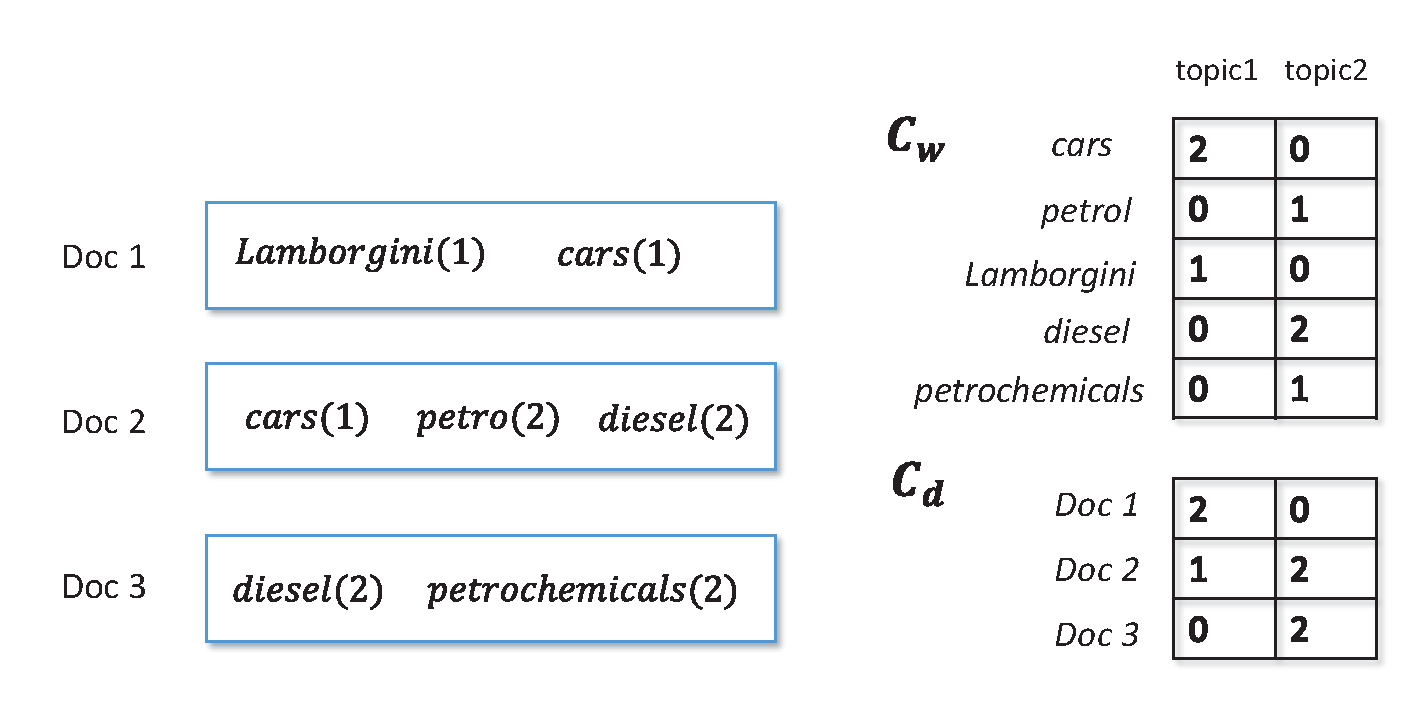
\includegraphics[width=0.8\linewidth]{figures/C_w_C_d.eps}\\
		\caption{An example for Corpus. The numbers in the parentheses
			are the current topic of each token. $\mathbf{C_w}$ and $\mathbf{C_d}$ contain counts of tokens that belong to a specific topic.}
		\label{fg:example}
	\end{figure}
	
	
\subsection{LDA Variants}
As the most popular topic model,
LDA is well known for its simplicity and efficient solution based on Gibbs sampling. 
However, its simplicity brings LDA some drawbacks that it is unable to cope with complex application scenarios. 
For instance, LDA cannot be used in supervised learning tasks where each document is assigned with labels, or the change of topics over time should be deduced.
To deal with certain complicated scenarios, many LDA variants have been proposed. 
Some of them add more information into LDA, e.g. Supervised Topic Model (STM), Topics over Time (TOT); some change the assumption of Dirichlet distribution, e.g. Correlated Topic Model (CTM). Here we introduce three classical topic models.

\subsubsection{Supervised Topic Models}
Supervised Topic Models (STM) adds a response variable associated with each document to the LDA model which can be either a continuous value for regression problems or a discrete value for classification problems.
STM jointly models the documents and the responses in order to explore topic distributions over documents more precisely as well as to predict the response variables of unlabeled documents.

Under STM model, each topic $k$ is a $V$-dim word distribution $\phi_k$, which follows a Dirichlet prior $\beta$; and each document $d$ and its response variable $y$ arises from the following generative process:
\begin{enumerate}
	\item Draw topic proportions $\theta_d \propto Dir(\alpha)$.
	\item For each token:
	\begin{enumerate}
		\item Draw topic assignment $z_{dn} \propto Mult(\theta_d)$.
		\item Draw word $t_{dn} \propto Mult(\phi_{z_{dn}})$.
	\end{enumerate}
	\item Draw response variable $y \propto \mathcal{N}(\eta^T \overline{z_d}, \sigma^2)$,\\
	where $\overline{z_d} = \frac{1}{L_d} \sum_{n=1}^{L_d} z_{dn}$ is the empirical topic frequencies and $z_{dn}$ is of one-hot representation.
\end{enumerate}
Similar with LDA, to generate a document $d$, STM first draws a $K$-dimentional topic mixing distribution $\theta_d$ from $Dir(\alpha)$, then draws
a topic assignment $z_{dn}$ from $Mult(\theta_d)$ followed by a word from $Mult(\phi_{z_{dn}})$ for each token $t_{dn}$. Beyond LDA, STM further draws a response variable $y$
based on the topic distribution of the document $d$ that is estimated by $\overline{z_d}$ in the model.

To inference an STM model, we should obtain the posterior
distribution of latent variables $(\Theta, \Phi, Z)$ as well as
the parameters of the normal distribution for response variables, $(\eta, \sigma^2)$. We apply the EM algorithm here
to do the inference process. The algorithm processes two steps
iteratively:
\begin{enumerate}
    \item Apply Collapsed Gibbs Sampling that integrates out $(\Theta, \Phi)$ 
    through conjugacy and sample  $z_{dn}$ for each token from 
    full conditional distributions just like that in LDA.
    \item Considering the sampling result $z_{dn}$ as an estimation of expectation of $Z$, we maximize the posterior log-likelihood $log~p(\eta|Z,W,Y,\alpha,\beta, \sigma^2)$ in terms of the parameter $\eta$.
\end{enumerate}
Similar with LDA, the core operation of the inference phase of STM is 
to assign topics for all tokens in $\mathcal{C}$ iteratively. It calculates probabilities for K topics according to the full conditional distribution of token $t_{dn}$ and picks one topic randomly:
\begin{align*}
\label{eq:slda_sampling}
p(&z_{dn} = k| t_{dn} = w, \eta, \sigma^2, \mathbf{Z}_{\neg dn}, \mathcal{C}_{\neg dn}) \propto
(C_{dk}^{\neg dn} + \alpha) ~ \\
&\frac{C_{wk}^{\neg dn} + \beta}{C_{k}^{\neg dn} + V\beta} ~
exp({-\frac{1}{2\sigma^2}
[\frac{\eta_k}{n}(2\eta^T\overline{z_{d,\neg n}}-2y_d-\frac{\eta_k}{n})]})
\end{align*}
\\
After the CGS step, the inference algorithm calculates the optimal value of $\eta$ to maximize the log-likelihood, which we denote as $\eta^*$.
\begin{align*}
\label{eq:slda_estimating}
log~p(\eta|Z,W,Y,\alpha,\beta, \sigma^2) \propto \sum_{d=1}^{M}{log~\mathcal{N}(\eta^T\overline{z_d}, \sigma^2)}
\end{align*}
\begin{align*}
\label{eq:slda_solution}
\eta^* = YZ(Z^TZ)^{-1}
\end{align*}

\subsubsection{Topics over Time}
Topics over Time model (TOT) plays an important role on
discovering topic evolution over time. This model 
assumes a continuous distribution over time associated 
with each topic, and topics are responsible for 
generating both observed timestamps as well as words. 
Under TOT model, each document arises from the following generative process:
\begin{enumerate}
	\item Draw topic proportions $\theta \propto Dir(\alpha)$.
	\item For each word
	\begin{enumerate}
		\item Draw topic assignment $z_n \propto Mult(\theta)$.
		\item Draw word $t_{dn} \propto Mult(\phi_{z_n})$.
		\item Draw timestamp $s_{dn} \propto Beta(\psi_{z_n})$.
	\end{enumerate}
\end{enumerate}
where $\phi_k$ is the word distribution for topic $k$ that is same as LDA and $Beta(\psi_{z_n})$ represents Beta distribution with parameters $\psi_{z_n,1}$ and $\psi_{z_n,2}$.

The generative process is similar with that of LDA model
and STM model, but unlike in STM that drawing a label for each document, TOT draws a timestamp for each token from Beta distribution with hyperparameter $\Psi$ based
on the associated topic. In practice, each document has
a timestamp and it is considered the observed timestamps of
all tokens in that document.

The inference algorithm for TOT is highly similar with that
for STM -- an EM based algorithm that doing sampling and
estimating parameters iteratively. In sampling step, we
apply CGS that integrates out $\Theta$ and $\Phi$ through
conjugacy and sampling $z_{dn}$ for each token from full
conditional distributions. In estimating step, we calculate
the optimal value of $\Psi$ to maximize the log likelihood $log~p(\Psi|Z,W,\alpha,\beta)$.

To process the core operation when inferencing a TOT model, we should calculate the full conditional distribution for each token $t_{dn}$ by:
\begin{align*}
\label{eq:tot_sampling}
p(z_{dn} = k&| s_{dn}, \mathbf{Z}_{\neg dn}, \mathcal{C}) \propto
(C_{dk}^{\neg dn} + \alpha) ~ \\
&\frac{C_{wk}^{\neg dn} + \beta}{C_{k}^{\neg dn} + V\beta}~
\frac{(1-s_{dn})^{\psi_{z_{dn},1}-1}s_{dn}^{\psi_{z_{dn},2}-1}}{B(\psi_{z_{dn},1},\psi_{z_{dn},2})}
\end{align*}
\\
where $B(\alpha,\beta)=\Gamma(\alpha)\Gamma(\beta)/\Gamma(\alpha+\beta)$. Afterwards, we calculate the optimal estimation $\Psi^*$ of $\Psi$ to maximize the log-likelihood:
\begin{align*}
\label{eq:tot_estimating}
log~p(\Psi|Z,W,S,\alpha,\beta) \propto \sum_{d=1}^{D}\sum_{i=1}^{L_d}{log~Beta(t_{di}|\psi_{z_{di},1}, \psi_{z_{di},2})}
\end{align*}
\begin{align*}
\label{eq:tot_solution}
&\psi_{z,1}=\overline{s_z}(\frac{\overline{s_z}(1-\overline{s_z})}{S_z^2}-1)\\
&\psi_{z,2}=(1-\overline{s_z})(\frac{\overline{s_z}(1-\overline{s_z})}{S_z^2}-1)
\end{align*}
where $\overline{s_z}$ and $S_z^2$ indicate the sample mean and the biased sample variance of the timestamps belonging to topic z, respectively.

\subsubsection{Correlated Topic Models}
Unlike LDA, Correlated Topic Models (CTM) adopts logistic normal distribution for topic proportions in order to exhibit correlation between topics. The generative process of each document $d$ turns to:
\begin{enumerate}
	\item Draw topic proportions $\theta_d \propto \mathcal{N}(\mu,\Sigma)$.
	\item For each word
	\begin{enumerate}
		\item Draw topic assignment $z_{dn} \propto Mult(f(\theta_d))$\\
		where $f(\theta_i)={exp\ \theta_i}/{\sum_j{exp\ \theta_j}}$.
		\item Draw word $t_{dn} \propto Mult(\phi_{z_{dn}})$.
	\end{enumerate}
\end{enumerate}
where the topic proportion $\theta_d$ is drawed from a normal distribution with hyperparameters $\mu$ and $\Sigma$, $\phi_k$ is the word distribution for topic $k$.

Because the prior topic distribution has been changed and normal distribution and multinomial distribution are not conjugate, we cannot use
CGS to integrate out $\Theta$. As a result, we 
should sample $\Theta$ in addition to $z_{dn}$ in the inference algorithm. Here we apply Stochastic Gradient Langevin Dynamics (SGLD) algorithm to sample continuous random variable $\Theta$.

SGLD is a  gradient based algorithm for sampling from continuous posterior distributions in the form that 
$p(\theta|X) \propto p(\theta)\prod_{i=1}^Np(x_i|\theta)$, 
where $X=\{x_i\}_{i=1}^N$ is a dataset. 
Let sequence $\{\epsilon_t\}$ satisfies: (1)$\sum_{t=1}^{\infty}\epsilon_t=\infty$; (2)$\sum_{t=1}^{\infty}\epsilon_t^2<\infty$. Then, beginning with any initial $\theta_0$, do the following iterative updates and $\theta_t$ will submit its posterior distribution after enough steps:
$$
\Delta \theta_t=\frac{\epsilon_t}{2}(\nabla log~p(\theta_t)+\frac{N}{n}\sum_{i=1}^{n}{\nabla log~p(x_{t,i}|\theta_t)})+\eta_t
$$
$$
\eta_t \propto \mathcal{N}(0,\epsilon_t)
$$
where $t$ denotes the step number. In each step, SGLD samples $n$ data items from $X$ randomly for consideration.

Therefore, we get a two-step sampler:
\begin{enumerate}
    \item Sample $z_{dn}$:
    \begin{align*}
    \label{eq:ctm_sampling_z}
    p(z_{dn} = k| t_{dn}, \mathbf{Z}_{\neg dn}, \mathcal{C}_{\neg dn}, \Theta) \propto\
    \frac{C_{wk}^{\neg dn} + \beta}{C_{k}^{\neg dn} + V\beta}~e^{\theta_{dk}}
    \end{align*}
    \item Sample $\Theta$:
    \begin{align*}
    \label{eq:ctm_sampling_theta}
    p(\Theta|\mathbf{Z},\mathcal{C}) \propto
    \prod_{d=1}^{M}{\{\mathcal{N}(\mu, \Sigma)\prod_{i=1}^{N_d}{\frac{e^{\theta_{d,z_{di}}}}{\sum_{k}{e^{\theta_{d,k}}}}}\}}
    \end{align*}
\end{enumerate}

\section{Sampler Selection}
	
	We study the system tradeoff of different
	samplers over four topic models---LDA, STM, TOT, and CTM; and propose a novel hybrid
	approach that automatically decides
	which sampler to use in different places.
	We start by presenting a taxonomy of
	four existing samplers, all of which
	were published recently.
	
	\subsection{Anatomy of Existing Samplers}
	\label{sec:samplers}
	
	\begin{figure*}[t]
		\centering
		\subfigure[doc length distribution]{
			\label{fg:length_distribution}
			% Requires \usepackage{graphicx}
			\scalebox{0.18}[0.18]{
				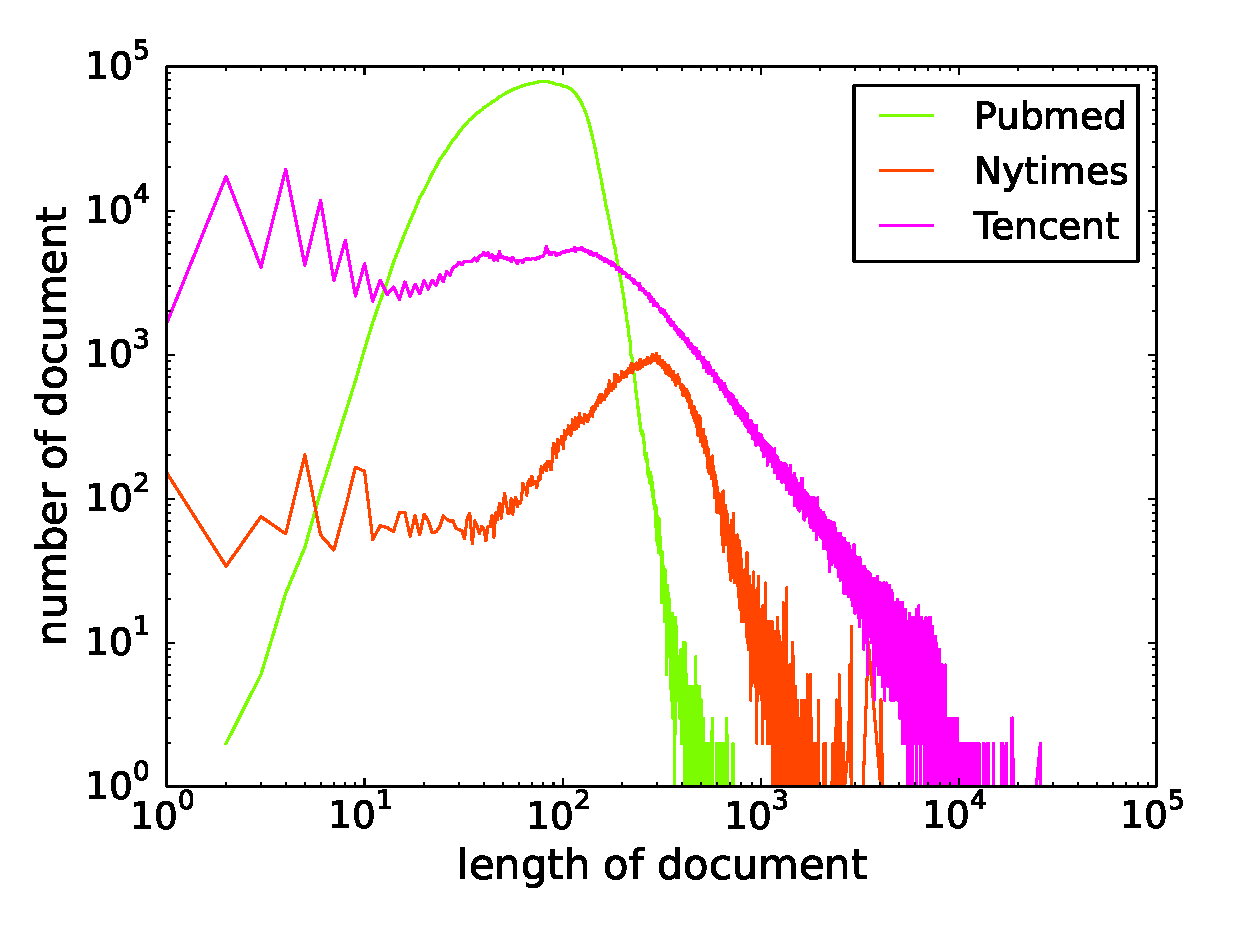
\includegraphics[width=\linewidth]{figures/length_dis.eps}
		}}
		\subfigure[K = 100]{
			\label{fg:length_K_100}
			% Requires \usepackage{graphicx}
			\scalebox{0.18}[0.18]{
				\includegraphics[width=\linewidth]{figures/topic_100.eps}
		}}
		\subfigure[K = 1k]{
			\label{fg:length_K_1k}
			% Requires \usepackage{graphicx}
			\scalebox{0.18}[0.18]{
				\includegraphics[width=\linewidth]{figures/topic_1k.eps}
		}}
		%\subfigure[\small K = 8k]{
		%  \label{fg:length_K_8k}
		%  % Requires \usepackage{graphicx}
		%  \scalebox{0.18}[0.18]{
		%  \includegraphics[width=\linewidth]{figures/topic_8k.eps}
		%  }}
		\subfigure[K = 16k]{
			\label{fg:length_K_16k}
			% Requires \usepackage{graphicx}
			\scalebox{0.18}[0.18]{
				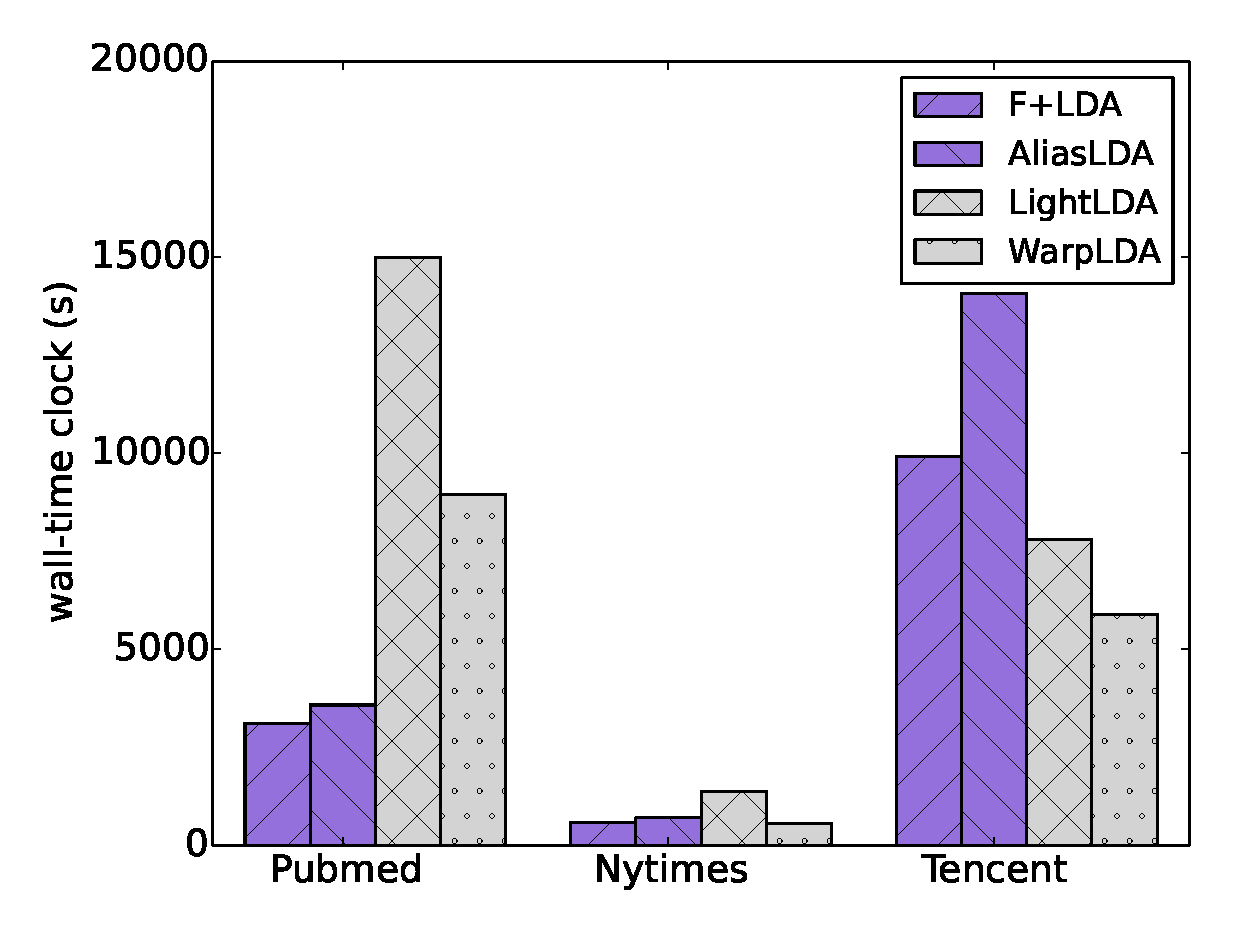
\includegraphics[width=\linewidth]{figures/topic_16k.eps}
		}}
		\subfigure[complexity over datasets]{
			\label{fg:complexity}
			% Requires \usepackage{graphicx}
			\scalebox{0.18}[0.18]{
				\includegraphics[width=\linewidth]{figures/complexity_ratio.eps}
		}}
		
		%\subfigure[\small number of samples to reach convergence]{
		%  \label{fg:accept_k_d}
		%  % Requires \usepackage{graphicx}
		%  \scalebox{0.19}[0.19]{
		%  \includegraphics[width=\linewidth]{figures/ll_over_samples.eps}
		%  }}
		%  \subfigure[\small complexity over samples]{
		%  \label{fg:accept_k_d}
		%  % Requires \usepackage{graphicx}
		%  \scalebox{0.19}[0.19]{
		%  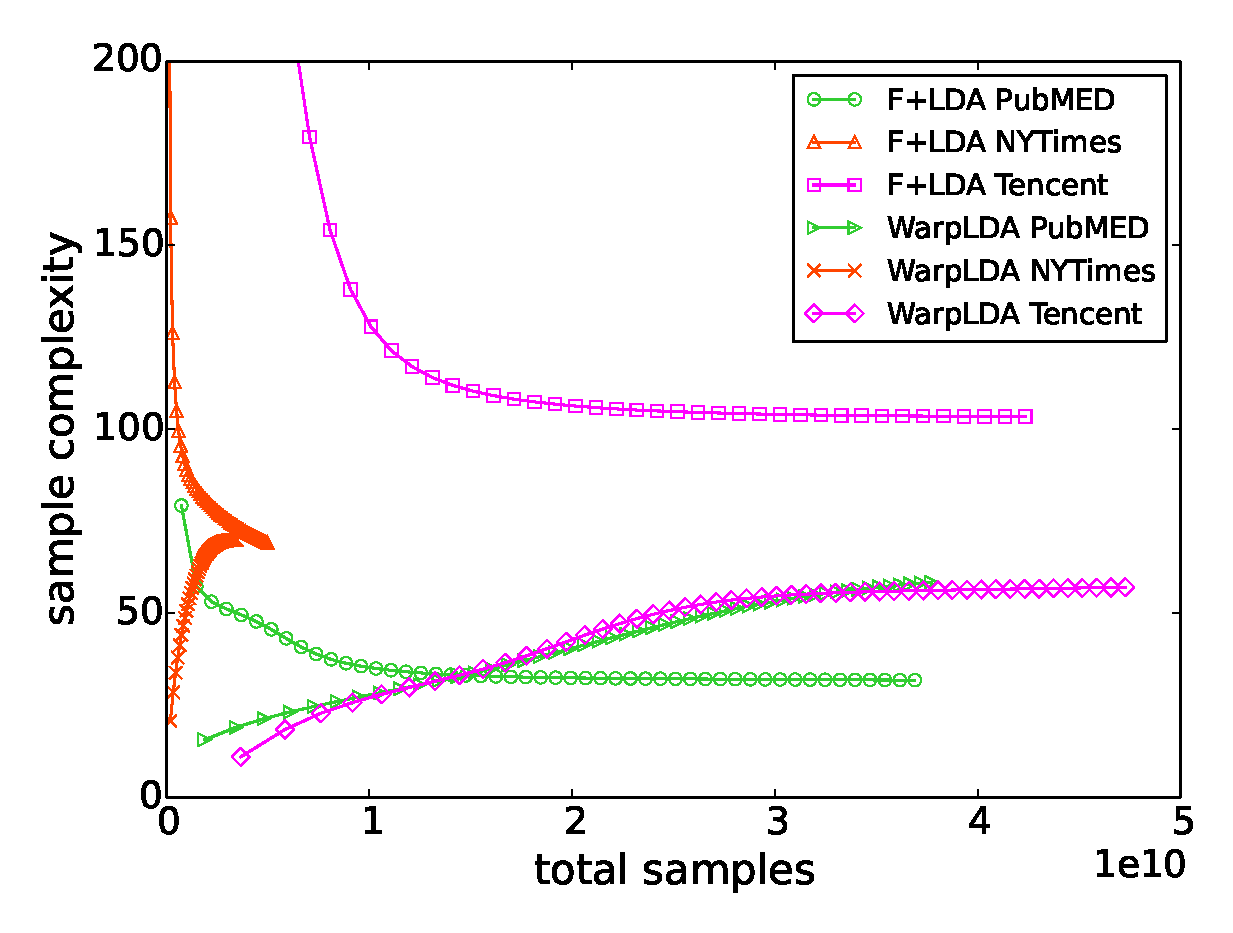
\includegraphics[width=\linewidth]{figures/complexity_over_samples.eps}
		%  }}
		\caption{Effects of document length and $K$ on the performance of samplers}
		\label{fg:summary}
	\end{figure*}
	
	Existing samplers can be classified
	into two categories according to the
	optimizations they use to reduce the sampling complexity:
	(1) {\bf SA samplers}, including
	AliasLDA and F+LDA, exploit the sparse structure of $\mathbf{C_d}$;
	and (2) {\bf MH samplers},
	including LightLDA and WarpLDA,
	use Metropolis-Hastings method to
	scale to a large number of topics.
	We study their tradeoff with the
	following experiment setup.
	\\

    \noindent
	{\large \em Settings}
	We implement all samplers under the same code base.
	For fair comparison, we optimize all these techniques and they are faster
	than all their original open-source implementations.\footnote{
		\scriptsize{\url{https://github.com/Microsoft/LightLDA},\url{http://bigdata.ices.utexas.edu/software/nomad/},\url{https://github.com/thu-ml/warplda}}}.
	All experiment results that we report are on a single machine and
	all samplers are parallelized with 16 threads.
	\\

    \noindent
	{\large \em Metrics} We measure the performance by the wall-clock time a sampler requires to converge to a given log likelihood value.
	We vary the number of topics and use datasets that have different
	characteristics to measure each sampler's
	performance.
	\\

    \noindent
	{\large \em Datasets} We use three different datasets to illustrate the tradeoff.
	One key characteristic turns out to
	be the length of a document, and the
	document length distribution is showed in Figure \ref{fg:length_distribution}.
	We see that these datasets have
	different length distribution---
	the PubMED dataset consists of
	many short documents whose length is less than 200, while the NYTimes dataset contains both short documents and long documents whose length can vary from 100 to 2000.
	For the Tencent dataset (the one from
	our industry partner), most of the tokens
	are from long documents with length larger than 1000---about 24\% of documents have a length over 1000, which contains more than 76\% of all tokens.
	

	\subsubsection{Sparse-Aware (SA) Samplers}
	
	AliasLDA and F+LDA decompose the
	probability for each token (Eq.~\ref{eq:lda}) into two parts: $C_{dk} \frac{C_{wk} + \beta}{C_k + V\beta}$ and $\alpha \frac{C_{wk} + \beta}{C_k + V\beta}$. When $C_{dk}$ ($\mathbf{C_{d}}$)
	is sparse, the sampler
	can skip those with zero $C_{dk}$, thus
	lowering the complexity.
	The difference between these two algorithms
	is the different data structures they use
	to perform sampling---AliasLDA uses the Alias table \cite{walker1977efficient}, while F+LDA uses the F+ tree.
	\\

    \noindent
	{\large \em Results}
	Figures~\ref{fg:length_K_100},~\ref{fg:length_K_1k}, and~\ref{fg:length_K_16k} show the results
	for different number of topics $K$.
	We can see that F+LDA is consistently faster than AliasLDA over all datasets and various values of $K$.
	The relative performances of AliasLDA and F+LDA are different across different datasets.
	Specifically, the gap becomes larger on the Tencent dataset, while it is much smaller
	on the other two datasets.
	This is because AliasLDA requires both traversal access and random access for $\mathbf{C_d}$ matrix, while F+LDA only requires traversal access. Since $\mathbf{C_d}$ is stored in sparse format---which aims to reduce memory cost---the latency of random access increases with more items in one document due to the increased conflicts in the hashtable.
	
	\subsubsection{Metropolis-Hastings (MH) Samplers}
	
	LightLDA and WarpLDA draw samples from two
	proposal distributions --- $q^{doc} \propto C_{dk} + \alpha$
	and $q^{word} \propto \frac{C_{wk} + \beta}{C_k + \beta}$ --- alternatively, and accept their proposals based
	on the acceptance condition of Metropolis-Hastings.
	These two samplers are different in their access
	order for the in-memory data structures---WarpLDA
	separates the access of tokens into two passes,
	where each pass only accesses $\mathbf{C_w}$
	or $\mathbf{C_d}$, respectively, in order to
	reduce random access.
	\\

    \noindent
	{\large \em Results}
	Figures~\ref{fg:length_K_100},~\ref{fg:length_K_1k},~\ref{fg:length_K_16k} show the results of MH Samplers.
	We see that WarpLDA is consistently faster than
	LightLDA. This is because WarpLDA effectively
	eliminates the amount of random accesses.
	The performance gap is influenced by the
	size of the vocabulary $|\mathcal{V}|$ --- the more words
	the corpus has, the more random accesses will be incurred
	by $\mathbf{C_w}$.
	For the PubMED dataset, which has the largest vocabulary,
	the performance gap between WarpLDA and LightLDA is largest;
	on the other hand, since the Tencent dataset only contains 88,916 distinct words in its vocabulary, this
	performance gap is relatively small.
	
	\subsection{Samplers for LDA variants}
	We have illustrated that sparse-aware or MH method can be used
	to further optimize Gibbs sampling for LDA model. In this 
	section, we discuss how to apply similar techniques on 
	LDA variants.
	
	\subsubsection{The effect of sampling order of SA samplers}
	In Preliminary section, we have discussed that Gibbs 
	sampling can draw the components in arbitrary order, i.e.
	we can sample $z_{di}$ with any order in LDA model. In practice,
	most implementations choose doc-first order or word-first order for
	less cache miss when sampling LDA model. When applying 
	doc-first order, the sampler draws topics for all tokens in one document before turning to another. Word-first order means that
	the sampler drawing topics for all tokens associated with one word at one time.
	
	Different sampling orders lead to different ways to utilize
	sparsity. Take F+LDA as an example. With word-first order, on can
	decompose the probability into $C_{dk} \frac{C_{wk} + \beta}{C_k + V\beta}$ and $\alpha \frac{C_{wk} + \beta}{C_k + V\beta}$ and maintain the values of $\{\frac{C_{wk} + \beta}{C_k + V\beta}\}_{k=1}^{K}$ in an F+Tree during sampling tokens of word $w$, then the sparsity of $C_{dk}$ can lower the complexity. On the other hand, with document-first order, the  probability should be decomposed into $C_{wk} \frac{C_{dk} + \alpha}{C_k + V\beta}$ and $\beta \frac{C_{dk} + \beta}{C_k + V\beta}$ so that $\frac{C_{dk} + \alpha}{C_k + V\beta}$ can  be maintained by FTree when sampling the tokens in a document. In this case the sparsity of $C_{wk}$ becomes the key of performance optimization.
	
	In general, since LDA variants are derived from LDA model, their models usually subject to similar distributions, e.g. Dirichlet distribution. Thus, they have factor $C_{dk}+\alpha$ or $C_{wk}+\beta$ in the full conditional distributions of their core operation.
	In the case of $C_{dk}+\alpha$, if the full conditional probability can be represented in the form of $(C_{dk}+\alpha)F(w,k)$  and given any $k_1 \not= k_2$, $F(w,k_1)$ and $F(w,k_2)$ share no common variable to be calculated, then we can lower the sampling complexity in the way of F+LDA that
	maintain the value $F(w,k)$ of each $k$ in an F+Tree and 
	decompose the probability into $C_{dk}F(w,k)+\alpha F(w,k)$ to skip those with zero $C_{dk}$.
	For example, in LDA,  $F(w,k)=\frac{C_{wk}+\beta}{C_k+V\beta}$, $C_{wk}$ and $C_k$ are variables which are satisfied that $C_{wk_1}$ and $C_{wk_2}$ are different variables, and so are $C_{k_1}$ and $C_{k_2}$. In addition, $V$ and $\beta$ are constants.
    In case of $(C_{wk}+\beta)$, we can obtain similar results in the same way.
	
	
	\subsubsection{Sampler for STM}
	
	\noindent
	{\large \em SA sampler} We first show how to adapt F+LDA to inference STM model. Consider the full conditional distribution to be calculated in the core operation of STM model. It almost conforms to $(C_{wk}+\beta)F(d,k)$ if we set 
	$F(d,k)$ to be $\frac{C_{dk}+\alpha}{C_{k}+V\beta}~
    exp(-\frac{1}{2\sigma^2}
    [\frac{\eta_k}{n}(2\eta^T\overline{z_{d,\neg n}}-2y_d-\frac{\eta_k}{n})])$, so we manage to optimize Gibbs sampling with the sparsity of word distribution in the doc-first sampling order. 
    
    The problem occurs in $\overline{z_d^{\neg n}}$ which makes $F(d,k)$ shares common variables over $k$.
    Consider $\overline{z_{dk}^{\neg n}}=C_{dk}^{\neg n}/N_d$, the values $C_{dk}^{\neg n}$ of all $k$ 
    are required by each $F(d,k)$. As a result, 
    F+Tree is not able to maintain the values $F(d,k)$ easily.
    
    To overcome this problem, we adopt MH method here:
    assume $\overline{z_{d}^0}$ is the value when document $d$ to be sampled, we adjust full conditional distribution by using $\overline{z_{d}^0}$ to replace $\overline{z_{d}^{\neg n}}$, then add an accept/reject step to offset the deviation we made in sampling: 
	$$F(d,k)=\frac{C_{dk}+\alpha}{C_{k}+V\beta}~
exp(-\frac{1}{2\sigma^2}
[\frac{\eta_k}{n}(2\eta^T\overline{z_{d}^0}-2y_d-\frac{\eta_k}{n})])$$
    $$Acceptance Rate: exp\{\frac{1}{\sigma^2}\frac{\eta_k}{N_d}\eta(\overline{z_{d}^{\neg n}}-\overline{z_{d}^0})\} $$
    Therefore we can consider $\overline{z_{d}^0}$ as
    constants in sampling step and apply F+LDA sampler
    to STM model.\\
    
    \noindent
    {\large \em MH Sampler} Then we consider how to adapt WarpLDA to STM model. The process is easy, with new proposal distributions $q^{doc}$ and $q^{word}$ , we can run WrapLDA directly:
    \begin{align*}
    &q^{word} \propto C_{wk}+\beta\\
    &q^{doc} \propto F(d,k)
    \end{align*}
    Here we continue to use $F(d,k)$ showed above, which allows sampler to draw topics in average $O(1)$ complexity.
	
	\subsubsection{Sampler for TOT}
	\noindent
	{\large \em SA sampler} To adapt F+LDA to TOT model, we observe that the full conditional distribution in the core operation of TOT is in form $(C_{wk}+\beta)F(d,k)$ where
	$$F(d,k)=\frac{C_{dk}+\alpha}{C_k+V\beta}~\frac{(1-s_{di})^{\psi_{k,1}-1}s_{di}^{\psi_{k,2}-1}}{B(\psi_{k,1},\psi_{k,2})}.$$
	Note that the timestamps $s_{di}$ of one
	document are of the same value and can be considered
	as a constant $s_d$ of a document. Therefore, we can optimize Gibbs sampling with the sparsity of word distribution in the doc-first sampling order. \\
	
    \noindent
    {\large \em MH Sampler} Similar with STM, we can set proposal distributions $q^{doc}$ and $q^{word}$ as follows and run WrapLDA
    directly to inference TOT models:
	\begin{align*}
    &q^{word} \propto C_{wk}+\beta\\
    &q^{doc} \propto F(d,k).
    \end{align*}
	
	\subsubsection{Sampler for CTM}
	\noindent
	{\large \em SA sampler} The full conditional distribution in the core operation of CTM also conforms $(C_{wk}+\beta)F(d,k)$ where
	$$
	F(d,k)=\frac{e^{\theta_{dk}}}{C_k+V\beta}.
	$$
	So we can adapt F+LDA to CTM model with the doc-first sampling order, which means sparsity of word distribution is in use. \\
	
    \noindent
    {\large \em MH Sampler} Again, similar with STM, we can set proposal distributions
	$q^{doc}$ and $q^{word}$ as
	\begin{align*}
    &q^{word} \propto C_{wk}+\beta\\
    &q^{doc} \propto F(d,k)
    \end{align*}
    and apply WarpLDA to CTM directly.
    
	\subsection{Tradeoff: SA vs. MH Samplers}
	We now describe the system tradeoff between SA
	and MH samplers. Because in our experiments
	F+LDA and WarpLDA always dominate others,
	we focus on the tradeoff between them.
	We first describe the tradeoff we observed, and
	then analyze it.
	\\

    \noindent
	{\large \em Summary of the Tradeoff}
	\begin{enumerate}
		\item \textbf{Length of Document $L_d$.}
		The length of documents turns out to be
		an important axis in the tradeoff. On
		datasets with many short
		documents, like PubMED, F+LDA
		is faster than WarpLDA---by up to 2.8$\times$ when $K = 16k$;
		(2) On datasets with many long
		documents, like Tencent,
		WarpLDA is faster than F+LDA---
		by up to 1.7$\times$ when $K = 16k$.
		
		\item \textbf{Frequency of Word $L_w$.} Words
		and documents play symmetrical roles in sampling
		processes. Although it is not easy to be observed 
		from natural datasets, we show results from two
		generated datasets A (few words but all with high frequency) and B (large number of words but all are low frequent). Both datasets are obtained by spliting NYTimes dataset into two
		parts.
		
		\item \textbf{Number of topics $K$.}
		The number of topics also plays a major role
		in the tradeoff. When the number of topics
		increases---e.g., from $1k$ to $16k$ on Tencent---
		WarpLDA becomes faster compared with F+LDA;
		Similarly, when the number of topics
		increases on PubMED, F+LDA becomes
		faster compared with WarpLDA.
	\end{enumerate}
	\\
	
	\noindent
	{\large \em Analysis.}
	The above tradeoff can be explained with
	the following analytical model.
	To generate one sample in WarpLDA,
	the Metropolis-Hastings sampler
	needs to decide whether to accept a
	sample or not. Let $\pi$
	be the acceptance rate, WarpLDA requires,
	in expectation, $\frac{1}{\pi}$ samples
	for one sample to be accepted. On the other
	hand, F+LDA does not have this overhead.
	However, to generate each sample,
	the computational complexity of F+LDA
	is $O(K_d)$ in word-first order or $O(K_w)$ in doc-first order, where $K_d$,
	the number of non-zero elements of $C_d$
	is bound by the number of topics $K$ and
	the length of a document $L_d$, or $O(K_w)$, where
	$K_w$, the number of non-zero elements of $C_w$,
	is bounded by the number of topics $K$ and the
	frequency of word $w$---$L_w$.
	On the other hand, WarpLDA incurs $O(1)$
	complexity to propose each sample.
	
	We can now see the tradeoff---when
	$K$, $L_d$, and $L_w$ are small, WarpLDA is
	slower because of its $\frac{1}{\pi}$
	overhead; otherwise, F+LDA is slower
	due to its overhead in generating each sample.
	
	The result we see in Figures~\ref{fg:length_K_100},~\ref{fg:length_K_1k},~\ref{fg:length_K_16k}
	is the result of an {\em aggregation}
	of the above analysis across the whole corpus.
	Figure~\ref{fg:length_distribution} illustrates
	the distribution of the length of documents.
	For the PubMED dataset, which consists of many
	documents with small $L_d$, F+LDA is faster
	than WarpLDA. For the Tencent dataset, which
	consists of documents with large $L_d$, WarpLDA
	is faster than F+LDA. For smaller $K$, F+LDA is
	faster than WarpLDA on all datasets.
	
	Figure~\ref{fg:complexity} further provides
	a quantitative illustration of the tradeoff.
	We define a {\em complexity ratio}
	$\lambda = K_d \pi$ as the ratio between
	the complexity of F+LDA and WarpLDA.
	As expected, on datasets
	where F+LDA is faster, $\lambda$ is smaller.
	This is consistent with the empirical
	result illustrated in Figure~\ref{fg:complexity}.
	
	\subsection{Hybrid Sampler}
	\label{sec:hybrid}
	
	The above tradeoff raises a natural question---
	{\em Can we build a hybrid sampler that marries
		both SA and MH sampler?} Intuitively, this
	is trivial---just run ``short" documents
	with F+LDA and ``long" documents with WarpLDA, or
	run ``special'' words with F+LDA and ``common'' words with WarpLDA.
	In practice, however, there are two
	technical questions: (1) how to decide
	which document is {\em long enough} or word is {\em common enough} to
	``qualify'' for WarpLDA; and (2)
	how to {\em balance} an MH sampler and an SA
	sampler, which have different convergence speeds.
	For the first question, we developed a very
	simple rule-of-thumb based on the study
	of our tradeoff. The second question is more
	challenging and ties to an open
	question in the mixing theory of two
	Markov chains. Inspired by classic statistical theory
	on a simpler underlying model, we develop a
	simple heuristics that works well across
	all of our datasets.
	
	In the following discussion, we assume that F+LDA runs in word-first order, i.e. decompose full conditional distribution
	into $C_{dk} \frac{C_{wk} + \beta}{C_k + V\beta}$ and $\alpha \frac{C_{wk} + \beta}{C_k + V\beta}$ so as to utilize the
	sparse structure of $C_{d}$. In the case of doc-first order,
	we can obtain similar results due to words and documents are
	symmetric roles in F+LDA---if we swap the terms ``document''
	and ``word'' in F+LDA, the sampler still works.
	
	\subsubsection{Sampler Selection}
	
	The first step is to design a rule-of-thumb to choose
	between two samplers. We focus on the combination
	of F+LDA and WarpLDA, as these two samplers dominate
	consistently faster than AliasLDA and LightLDA
	in our tradeoff study.
	\\

    \noindent
	{\large \em Sampling Complexity}
	For F+LDA to generate one sample, it needs to traverse
	the non-zero items in $C_{dk}$, whose size is bounded by $K$ and $L_d$.
	Thus, the sampling complexity of F+LDA is
	\begin{displaymath}
	C_{f+} = O(min(L_d, K))
	\end{displaymath}
	On the other hand, since Metropolis-Hastings method requires mix time for each sample,
	the complexity of WarpLDA is
	\begin{displaymath}
	C_{wrap} = O(n)
	\end{displaymath}
	where $n$ is the steps to achieve mix.
	
	The technical challenge is how to estimate $n$, whose value not only
	depends on the input datasets, but also changes across iterations. In theory,
	estimating the {\em mixing time} of
	the underlying MCMC chain for general factor graphs is a problem
	that has been around for decades. With this in mind, we resort to
	a simple heuristics that is motivated by the empirical
	observation from our study.\\
	

	\noindent
	\textbf{Heuristics 1 (word-first order).} Given a document $d$ with length $L_d$ and topic number $K$, if $K \le S$ or $L_d \le S$ choosing F+LDA;
	otherwise, choosing WarpLDA.
	$S$ is a threshold value that depends on the implementation and properties of the dataset.
	\\
	
	\noindent
	\textbf{Heuristics 1 (doc-first order).} Given a word $w$ with frequency $L_w$ and topic number $K$, if $K \le S$ or $L_w \le S$ choosing F+LDA;
	otherwise, choosing WarpLDA.
	$S$ is a threshold value that depends on the implementation and properties of the dataset.
	
	\subsubsection{Balancing Two Chains}
	
	One surprising observation is that the above heuristics itself is not
	enough for a hybrid sampler that outperforms both F+LDA and WarpLDA.
	The fundamental reason is that two Markov chains underlying F+LDA and WarpLDA
	{\em do not converge with the same speed}.
	Specifically, all samples from F+LDA will be accepted, however this is not the case for WarpLDA.
	Intuitively, this means that a naive hybrid sampler would generate more samples
	for tokens belonging to F+LDA per epoch than WarpLDA.
	\\
	

    \noindent
	{\large \em Theoretical Understanding} The above observation raises a fundamental
	question: {\em What is the relationship between the mixing time of a
		Gibbs sampler (F+LDA) and a Metropolis-Hastings (WarpLDA) sampler for the
		same underlying distribution?} If we {\em magically} know the ratio
	between their mixing time, we could just use this number to balance these
	two chains.
	
	Unfortunately, a general treatment of this question has existed for
	decades and is still under intensive study by the theoretical computer
	science and mathematics community. However, there are theoretical
	results that can be used to {\em inspire} our practical heuristics.
	
	We know that the mixing time of these two chains is not too different,
	at least for Ising model:
	

	\begin{lemma}~\cite{levin2009markov}(Levin, Peres, \& Wilmer 2008, Example 13.18)
		For a graph with vertex set $V$, let $\pi$ be the Ising
		probability measure. Let $\gamma$ be the spectral gap
		of the Gibbs chain and $\tilde{\gamma}$ be the spectral gap
		of the Metropolis chain using the base chain, we have
		\[
		\gamma \le \tilde{\gamma} \le 2\gamma
		\]
	\end{lemma}
	where $\gamma$ is related to the mixing time
	by the following lemma

	\begin{lemma}~\cite{levin2009markov}(Levin, Peres, \& Wilmer 2008, Theorem 12.3)
		Let $P$ be the transition matrix of a reversable, irreducible
		Markov chain with state space $\Omega$, and $\pi$ be the
		underlying probability measure. Let $\pi_{min} = \min_{x\in \Omega} \pi(x)$
		and $\gamma$ the absolute spectral gap (equals to the spectral gap
		when the chain is ``lazy''), we have the mixing time
		\[
		t_{min}(\epsilon) \le \log(\frac{1}{\epsilon \pi_{min}})\frac{1}{\gamma}
		\]
	\end{lemma}
	
	The above two lemmas inspired the design in two ways.
	First, we know, at least intuitively, whatever scheme
	we use to balance these two chains, that scheme should
	not be ``too extreme'' (these two chains are off by a
	constant factor anyway). Second, the mixing time is
	likely to be linear (or inverse linear) to the constant
	that we will use to balance these two chains. Inspired
	by these, our simple heuristics is as follows:\\
	

	\noindent
	\textbf{Heuristics 2.} For each epoch, the MH steps for the WarpLDA
	is set to $\lceil\frac{1}{\pi}\rceil$,
	where $\pi$ is the acceptance rate for the last epoch.\\
	

	The intuition behind this heuristics is simple---just use
	the empirical acceptance rate $1 / \pi$ as the proxy for
	the ratio of spectral gap $\frac{\tilde{\gamma}}{\gamma}$
	(In extreme cases where all MH samples are accepted ($\pi=1$),
	MH becomes Gibbs, and therefore $\frac{\tilde{\gamma}}{\gamma}=\frac{1}{\pi}$
	in this extreme case.)
	
	
	
	\begin{figure}[t]
		\center
		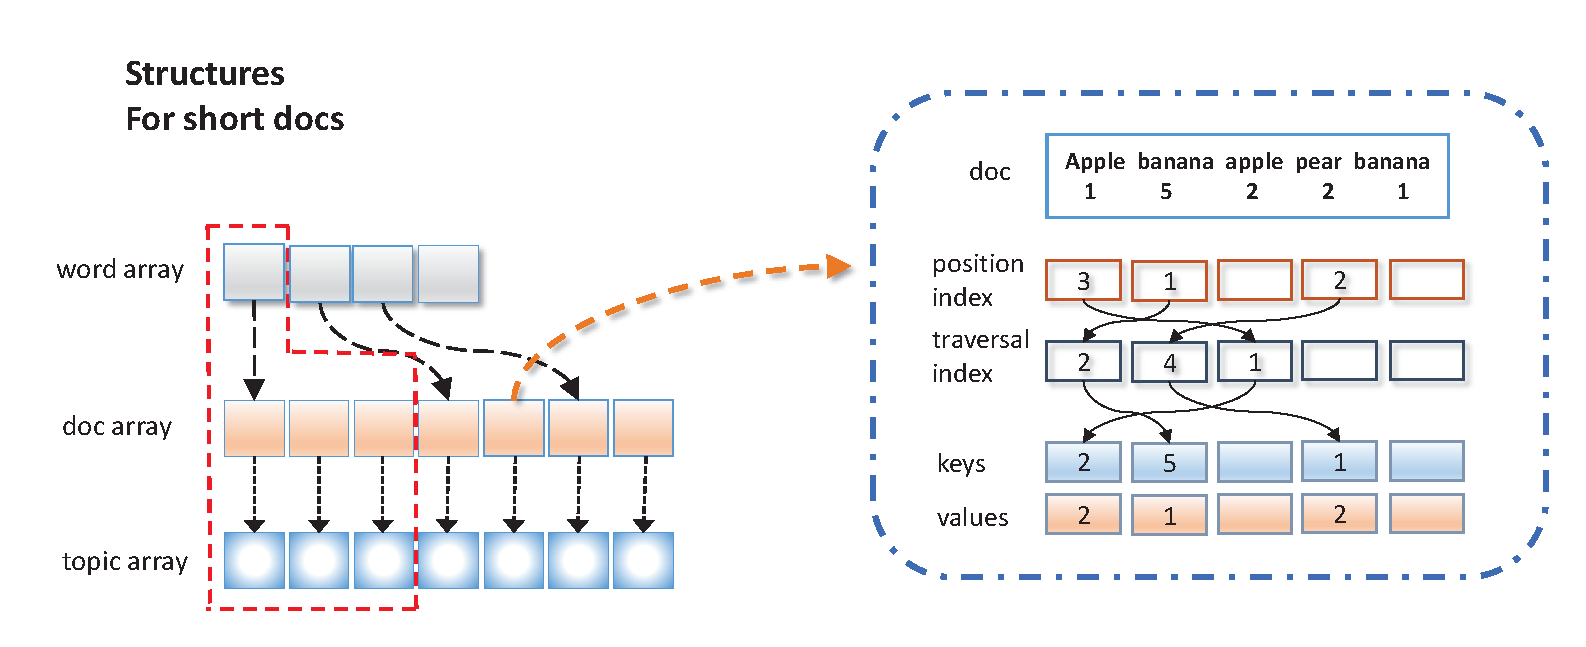
\includegraphics[width=0.9\linewidth]{figures/short_docs.eps}
		\caption{data structures for short docs.}
		\label{fg:short_docs}
	\end{figure}
	\begin{figure}[t]
		\center
		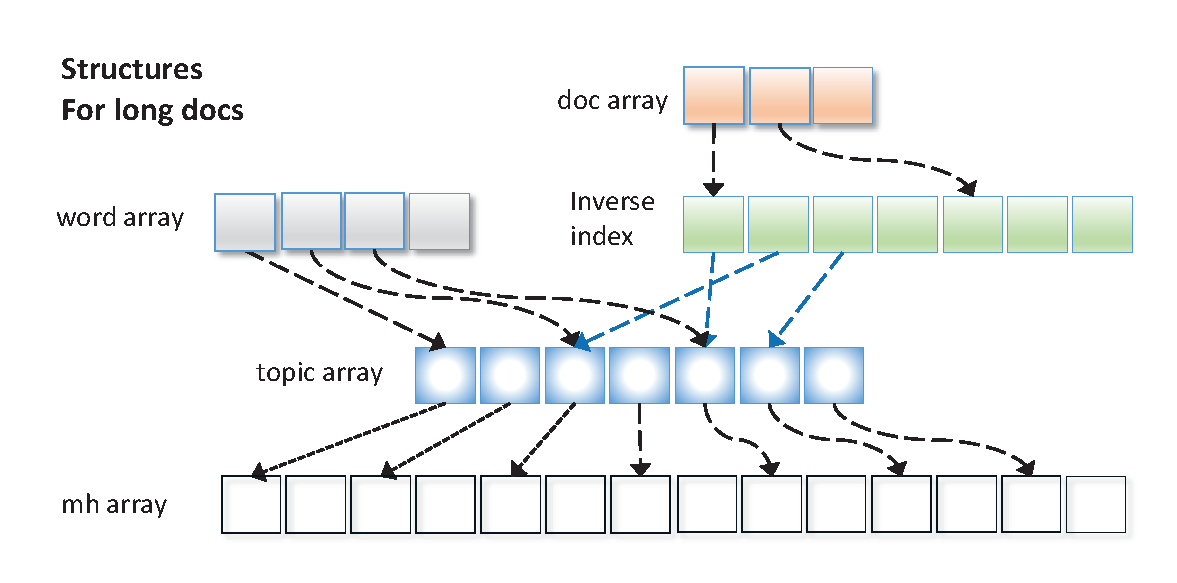
\includegraphics[width=0.9\linewidth]{figures/long_docs.eps}
		\caption{data structures for long docs.}
		\label{fg:long_docs}
	\end{figure}
	
	\section{System Implementation}
	In this section, we present a novel topic model system
	Liblda and its implementation details. Liblda provides
	users fully functions that stores/loads corpus data,
	training topic models and saving the results, and inferring
	new corpus based on pre-trained models. Liblda is implemented
	by C++ and supports all topic models we introduced in this paper---LDA, STM, TOT, and CTM. To obtain good performance, 
	all inference algorithms are based on the hybird sampler we presented 
	in section 4. 
    With Liblda, users can not only train and inference topic models  with fast algorithm very simply, they can 
    also implement new inference algorithms for other topic models under the algorithm framework in Liblda very easily.
    
    \subsection{System Architecture}
    We first present the architecture of Liblda. The goals of Liblda are
    (1) for users who treat topic models as black-boxes, they can 
    complete loading their data set, training an pre-implemented topic model, and getting results in ten lines; (2) for users who want to implement 
    new inference algorithms for other topic models, they can implement
    a high performance algorithm easily by extending an existing algorithm
    framework. In general, Liblda maintains three main parts of data: Corpus , Model, and Result.
    A Corpus is a set of documents that each contains a number
    of words. Sometimes documents are labeled with additional 
    information such as timestamps or category IDs. A Model
    is an instance of a topic model, in which records a set of parameter values and topic-word counters that can be used to inference new corpus data.  
    Users can train a model over a corpus or inference a corpus with a pre-trained model, and both actions come up with a Result instance. 
    A Result keeps topic distributions got by training or inference process for all documents involved.
    
    \vspace{0.5em}
    \noindent
    {\bf (Corpus in Liblda)} Corpus class in Liblda is to 
    represent document sets. Inside a Corpus, each document and each word has an unique integer identifier, and everything is stored with those integer IDs and tokens are stored in either doc-by-doc order or word-by-word order, which is
    determined by the user so that the inference algorithm can access the documents with proper order for
    cache efficiency. There also maintains an index mapping between two orders for convenience. Besides tokens, a Corpus
    also records a vector of arbitrary integer and float values for each document that can stored additional document information. Such design
    guarantees that a Corpus can represent broad enough kinds of data sets,
    and is easy to use by different sampling algorithms. \\
    
    \vspace{0.5em}
    \noindent
    {\bf (Model in Liblda)} Model class in Liblda is a virtual  class to represent topic models. 
    It defines basic interfaces: Train(Corpus), Inference(Corpus), Save(path), and Load(path). 
    All topic models have their own implementations of basic Model class that has different model parameters and inference algorithms. 
    All topic models in this paper have been implemented in Liblda: LdaModel, SLdaModel, TotModel, and CtmModel. 
    Users can easily creates a new Model instance by specifying the
    value of that model's hyper parameters, then train that model with a Corpus. 
    After training, the Model will contains results of topic-word distributions as well as other parameter values of that model. 
    Users can apply the trained model on a new Corpus to inference doc-topic distributions of the documents in that Corpus or save the Model and use it in the future. 
    In addition, users can do incremental training in Liblda---to train a model further with another Corpus. 
    The Train and Inference methods are implemented with high performance
    hybird samplers. In section 5.2, we will see how to easily implement a new  inference algorithm with our framework and obtain high performance
    with our advanced hybird sampler.\\
    
    \vspace{0.5em}
    \noindent
    {\bf (Result in Liblda)} Result class in Liblda is to
    represent training or inference results over a corpus.
    It contains topic distributions of all documents in
    a corpus. After {\em Train} or {\em Inference} API 
    of {\em Model} class is executed, a Result comes out.
    Users can easily access the results in it and store them into
    a file.
    
    \subsection{Algorithm Framework}
    Here we present a sampling based framework of inference algorithm for LDA model and its variants. This framework is based on expectation maximization(EM) algorithm that can be used to inference all topic models in this paper and can be easily extended to inference other models with proper attributes. We suppose a model can be inferenced by two steps: sampling from a posterior distribution (Sampling step) and estimating parameters (Estimating step). In Sampling steps, an algorithm should sample topics for all tokens in
    a Corpus and sometimes should sample other variables from
    some continuous distributions. For sampling topics, we
    apply our hybird samplers---with the sparsity of a model,
    we split the whole Corpus into two parts based on document
    lengths or word sizes, then sample tokens in the two parts separately with F+LDA sampler or WarpLDA sampler. 
    Besides, we apply SGLD algorithm to sample continuous variables. 
    In Estimating steps, the algorithm computes the optimal parameter values to maximize the log likelihood with current sampling results. 
    The algorithm repeats Sampling step and Estimating step iteratively until the log likelihood is coverage.
    
    To implement a new algorithm based on our framework, users only need
    to extend basic Model class by defining model specific parameters (including the traverse order of F+LDA sampler) and implementing their own SampleOtherVariables() and EstimateParameters() as well as model specific functions inside HybirdSampler() such as Initialize(), 
    FTreeValue(), SamplingWithFTree(), DocPropose(),  WordAcceptanceRate(), etc.
    For more details please visit our project documentations.
    
	\begin{algorithm}[t]
		\DontPrintSemicolon
		\SetKwFunction{FMain}{Train(corpus)}
		\SetKwProg{Fn}{Function}{}{}
		\Fn{\FMain}{
		    // Initialize distributions and parameters \\
		    $Initialize(corpus)$\\
		    // Running EM steps iteratively until converge \\
			\For{$iteration \leftarrow 1$ \KwTo $I$} {
			    // Running hybird sampler to sample topic \\
			    // assignments for each token\\
			    $HybirdSampler(corpus)$	\\
			    // Sampling other random variables using\\
			    // Gibbs sampling or SGLD\\
			    $SampleOtherVariables(corpus)$\\
			    // Estimating parameters in the model by\\
			    // maximizing the posterior loglikelihood\\ $EstimateParameters(corpus)$
			}
		}
		\caption{Algorithm Framework}
		\label{alg:framework}
	\end{algorithm}
    
	\subsection{Sampler Implementation}
	
	We now present the implementation of our hybrid sampler.
	We design different data structures for both F+LDA and WarpLDA
	since they have different access patterns. Our
	implementation for F+LDA is actually faster than
	the original F+LDA paper---in order
	to obtain $O(min(K, L_d))$ complexity for F+LDA, the structure
	for short documents requires careful design, since
	the cost for traversing a hashmap is proportional to the size
	of it, which can be larger than $K$ or $L_d$.
	Therefore, we build an extra index to guarantee achieving the
	theoretical complexity for F+LDA.
	\\

    \noindent
	{\large \em Structure for Short documents}
	Figure \ref{fg:short_docs} shows the structure for short documents, which is constructed by the CSC format for accessing tokens and a set of hashmaps for accessing $C_{dk}$.
	The index is built to accelerate the traversal of non-zero items for each row of $\mathbf{C_d}$,
	which can guarantee the complexity of F+LDA is $O(min(K, L_d))$ rather than the size of a hashmap.
	Since $C_{dk}$ can be updated after each sampling operation, we allocate one more ``position array'', which records the position of each key in the index array, in order to obtain an $O(1)$ maintenance complexity for each update operation.
	To reduce the memory introduced by the extra index, we use different data types to store these two arrays for different documents.
	Specifically, if $L_d \le 256$, we use the Byte type to store them.
	Otherwise, the Short type is chosen.
	\\
    
    \noindent
	{\large \em Structure for Long documents}
	For long documents, the structure is the same as WarpLDA, which is presented in Figure \ref{fg:long_docs}.
	Three arrays, including word array, doc array, and inverse index, are allocated to support both
	the ``document pass'' and the ``word pass'' for tokens.
	The topic array stores the topic assignment and the MH array maintains the MH proposals for each token.
	The difference is that we employ this structure to visit tokens only from long documents, while WarpLDA builds it to traverse all tokens.
	\\
	
	\noindent
	{\large \em Parallel Execution}
	Since the original F+LDA and WarpLDA use different parallelization strategies, we combine them sequentially in a coarse granularity---we first sample tokens from short documents with
	F+LDA, then use WarpLDA to sample tokens from long documents.
	Algorithm \ref{alg:parallel_sampler} shows the details.
	
	\begin{algorithm}[t]
		\DontPrintSemicolon
		\SetKwFunction{FMain}{HybirdSampler(corpus)}
		\SetKwFunction{FIsLongDoc}{IsLongDoc}
		\SetKwProg{Fn}{Function}{}{}
		\Fn{\FMain}{
			$ShortSet$, $LongSet$ $\leftarrow$ split $corpus$ through Heuristics 1\;
			$ShortDS$, $LongDS$ $\leftarrow$ build($ShortSet$), build($LongSet$) \;
			$mh_a = 2; mh_g = 2$\;
			\For{$iteration \leftarrow 1$ \KwTo $I$} {
				// Sampling short docs using F+LDA \;
				
				\For{$w \leftarrow 0$ \KwTo $V$}{
					\For{$token~t_{d,w}$ belongs to $w$ from $ShortDS$} {
						lock(d)\;
						Perform sampling operation\;
						unlock(d)\;
					}
				}
				
				// Sampling long docs using WarpLDA\;
				
				$\pi \gets$ Word pass on $LongDS$\;
				$mh_a = mh_g; mh_g = \lceil\frac{1}{\pi}\rceil$\;
				
				$\pi \gets$ Doc pass on $LongDS$\;
				$mh_a = mh_g; mh_g = \lceil\frac{1}{\pi}\rceil$\;
			}
		}
		\caption{Parallel Execution for Hybrid Sampler}
		\label{alg:parallel_sampler}
	\end{algorithm}
	
	At the start of training, we initialize two MH steps, including $mh_a$ and $mh_g$, which indicate the MH steps for the proposal accepting phase and the MH steps for the proposal generating phase in WarpLDA.
	We choose 2 as the default value for both of them since $\pi$ is always less than 1.
	For each iteration, we first visit short documents through F+LDA in parallel and then sample tokens from long documents through WarpLDA.
	We parallelize the training of F+LDA over word and lock on the access of $\mathbf{C_d}[d,]$ before the sampling operation.
	The lock operation aims to prevent concurrent write operations for the same row of $\mathbf{C_d}$.
	For long documents, the parallelization is achieved by paralleling over words in the word pass and paralleling over docs in the document pass.
	After each pass, we calculate the value of $\pi$ for it and change $mh_a = mh_g, mh_g = \lceil\frac{1}{\pi}\rceil $.
	
\section{Evaluation}
\label{sec:evaluation}

In this section, we report experiments results of
three parts: (1) we show results validating our
technical contribution of system tradeoffs;
(2) we evaluate our hybird LDA sampler and compare
it with state-of-the-art systems for LDA; 
(3) we compare our hybird samplers for STM, TOT, 
and CTM with the sampling methods derived from
F+LDA and WrapLDA.
Our technical contributions, including system tradeoffs and hybird samplers for different topic models, significantly improve the performance of our system.

\subsection{Experimental Setup}

\begin{table}[t]
	\caption{Dataset Statistics}
	\begin{tabular}{crrrrr}
		\hline
		\textbf{dataset} & \textbf{\#docs} & \textbf{\#words} &\textbf{\#tokens}
		& \tabincell{l}{\textbf{average} \\ \textbf{doc} \\ \textbf{length}}
		& \tabincell{l}{\textbf{sparse} \\ \textbf{text} \\ \textbf{size}}\\
		\hline
		\hline
		NYTimes  & 300K & 102660  & 99M  & 331 & 1GB \\
		\hline
		PubMED   & 8.2M & 141044  & 737M & 90 &  4GB \\
		\hline
		Tencent  & 2.5M & 88916   & 1.26B & 504 & 5.6GB \\
		\hline
		BaiKe    & 2.8M & 98234   & 418M  & 148   & 2.3GB \\
		\hline
	\end{tabular}
	\label{tb:dataset}
\end{table}
\\

\noindent
{\large \em Datasets}
Table~\ref{tb:dataset} summarizes the datasets we used.
We use four datasets, including NYTimes, PubMED, Tencent, and BaiKe, to evaluate the speed of samplers.
Compared with the other three datasets, BaiKe is a dataset with many long documents as well as many short documents.
NYTimes and PubMED are public
datasets\footnote{\scriptsize https://archive.ics.uci.edu/ml/machine-learning-databases/bag-of-words/}, while the other datasets are from our industry partner.\\

\noindent
{\large \em Experiment Setting}
We conduct all experiments on a
server which has an Intel Xeon E5530 @ 2.4G CPU with
16 cores, 74GB DDR3 memory and 10$\times$2TB SATA
hard disks. Following prior arts, we set the hyperparameter of Dirichlet distribution $\alpha=\frac{50.0}{K}$ and
$\beta=0.01$ for all the following experiments.

In all experiments, we run our own implementations of F+LDA and WrapLDA, as well as their adapted versions
for STM, TOT, and CTM.  We conduct two sets of
experiments. First, we validate system tradeoffs in
four topic models. We validate the tradeoff of $L_d$ and $K$
in LDA, and tradeoffs of $L_w$ and $K$ in STM, TOT, and CTM.
To validate the tradeoffs of $L_d$ and $L_w$, we 
conduct datasets with different ranges of document lengths or word frequencies. 
To validate the tradeoff of $K$, we set different topic
numbers and run experiments with the same dataset.
Then we evaluate the performance of our hybird 
samplers of the four topic models by comparing them
with F+LDA and WrapLDA. To compare the performance
among F+LDA, AliasLDA, WrapLDA, and LightLDA, we
implement all of them for LDA and report the results. We conduct experiments for LDA with all four datasets and for STM, TOT, and CTM we conduct experiments
with NYTimes and PubMED. We generate timestamps 
for all documents randomly in experiments of STM
and TOT.\\

\noindent
{\large \em Metrics}
We measure the quality of a topic model by the log
joint likelihood.
We count the wall-clock time for a method to reach a given loglikelihood value in order to compare their performance.
In our experiments, we measure four topic models---LDA,
STM, TOT, CTM. The log joint likelihood is calculated
by:
\begin{align*}
L_{LDA} &= log~p(W, Z|\alpha, \beta) = log \prod_d [\frac{\Gamma(\overline \alpha)}{\Gamma(\overline \alpha + L_d)}\\
&\prod_k \frac{\Gamma(\alpha_k + C_{dk})}{\Gamma(\alpha_k)}]
 \prod_k [\frac{\Gamma(\overline \beta)}{\Gamma(\overline \beta + C_k)} \prod_w \frac{\Gamma(\beta + C_{wk})}{\Gamma(\beta)}]\\
L_{STM} &= log~p(W, Z, Y|\alpha, \beta, \eta, \sigma^2) \propto \\
lo&g \prod_d \prod_k \Gamma(\alpha_k + C_{dk}) \prod_k [\frac{\Gamma(\overline \beta + C_{wk})}{\Gamma(\overline \beta + C_k)} \prod_d \mathcal{N}(\eta^T\overline{z_d}, \sigma^2)\\
L_{TOT} &= log~p(W, Z, T|\alpha, \beta, \Psi) \propto \\
lo&g \prod_d \prod_k \Gamma(\overline \alpha_k + C_{dk})
 \prod_k [\frac{\Gamma(\overline \beta + C_{wk})}{\Gamma(\overline \beta + C_k)} \\
 &\prod_d \prod_{i} Beta(t_{di}|\Psi_{z_{di},1}, \Psi_{z_{di},2})\\
L_{CTM} &= log~p(W, Z, \Theta |\alpha, \beta, \mu, \Sigma) \propto log \prod_d [\mathcal{N}(\theta_d|\mu,\sigma^2)\\
&\prod_i \frac{e^{\theta_d^{z_{di}}}}{\sum_j{e^{\theta_d^j}}}]
\prod_k [\frac{1}{\Gamma(\overline \beta + C_k)} \prod_w \Gamma(\beta + C_{wk})]
\end{align*}\\

\begin{table}[t]
	\caption{Wall-clock time (seconds) for samplers to reach the same log likelihood.}
	\begin{tabular}{|c|r|r|r|r|r|r|}
		
		\hline
		\textbf{dataset} & \textbf{K\& L} & \textbf{F+} &\textbf{Alias}
		& \textbf{Light}
		& \textbf{Warp}
		& \textbf{Hybrid}\\
		\hline
		\hline
		\multirow{3}{*}{PubMED} & 1k\&-6.6e9 & 2489  & 2865  & 11024 & 4400 & \textcolor{blue}{2322}\\
		\cline{2-7}
		& 8k\&-6.7e9 & 2851  & 3355 & 13045 & 7389 & \textcolor{blue}{2212} \\
		\cline{2-7}
		& 16k\&-6.8e9 & 3115  & 3580 & 15426 & 8957 & \textcolor{blue}{2713}\\
		\hline
		\hline
		\multirow{3}{*}{NYTimes}& 1k\&-9.7e8 & 712   & 879  & 1600   & 750 & \textcolor{blue}{431}\\
		\cline{2-7}
		& 8k\&-1e9 & 706 & 781  & 1760 & 761 & \textcolor{blue}{592} \\
		\cline{2-7}
		& 16k\&-1e9  & 589  & 709   & 1377 & 554 & \textcolor{blue}{403}\\
		\hline
		\hline
		\multirow{3}{*}{Tencent} & 1k\&-9e9 & 3500  & 5108   & 3564 & 3087 & \textcolor{blue}{2142}\\
		\cline{2-7}
		&8k\&-9e9 & 7746  & 11839   & 7500 & 4747 & \textcolor{blue}{4341}\\
		\cline{2-7}
		&16k\&-9e9 & 9910 & 14072   & 7800 & 5894 & \textcolor{blue}{5773}\\
		\hline
		\hline
		\multirow{2}{*}{BaiKe} & 8k\&-3.6e9 & 1893  & 2505   &  3308& 2045 & \textcolor{blue}{1158}\\
		\cline{2-7}
		& 16k\&-3.6e9 & 2763  &  3065  & 6930 & 3792 & \textcolor{blue}{1779}\\
		\hline
	\end{tabular}
	\label{tb:wall_time}
\end{table}

\begin{table}[t]
	\caption{Wall-clock time (seconds) for samplers to reach the same log likelihood.}
	\begin{tabular}{|c|r|r|r|r|r|}
		\hline
		\textbf{model} & 
		\textbf{dataset} & 
		\textbf{K\& L} & 
		\textbf{Warp} &
		\textbf{F+} &
		\textbf{Hybrid}\\
		\hline
		\hline
		\multirow{6}{*}{STM} &
		\multirow{3}{*}{Tencent} & 1k\&1.1e9 & 4242  & 2568 & \textcolor{blue}{2518}\\
		\cline{3-6} & & 2k\&1.9e9 & 5518  & 3211 & \textcolor{blue}{2854}\\
		\cline{3-6} & & 3k\&3.0e9 & 6776  & 4851 & \textcolor{blue}{3457}\\
		\cline{2-6} & \multirow{3}{*}{NYTimes} & 1k\&8.1e8 & 1461  & \textcolor{blue}{389} & 660\\
		\cline{3-6}& & 2k\&2.5e9 & 1912  & 987 & \textcolor{blue}{701}\\
		\cline{3-6}& & 3k\&4.4e9 & 2303  & 1221 & \textcolor{blue}{878}\\
		\hline
		\hline
		\multirow{6}{*}{TOT} &
		\multirow{3}{*}{Tencent} & 3k\&7.2e9 & 5121  & 9892 & \textcolor{blue}{3315}\\
		\cline{3-6} & & 5k\&1.3e10 & 7436  & 23079 & \textcolor{blue}{3979}\\
		\cline{3-6} & & 8k\&2.2e10 & 12492  & 50773 & \textcolor{blue}{6167}\\
		\cline{2-6} & \multirow{3}{*}{NYTimes} & 3k\&4.9e9 & 888  & 390 & \textcolor{blue}{358}\\
		\cline{3-6}& & 5k\&9.1e9 & 1129  & 1206 & \textcolor{blue}{601}\\
		\cline{3-6}& & 8k\&1.5e10 & 1504  & 2076 & \textcolor{blue}{715}\\
		\hline
		\hline
		\multirow{6}{*}{CTM} &
		\multirow{3}{*}{Tencent} &
		1k\&-6.6e9 & 4404  & 10612 & \textcolor{blue}{4169}\\
		\cline{3-6}& & 2k\&9.7e8 & 5632  & 13613 & \textcolor{blue}{5139}\\
		\cline{3-6}& & 3k\&1.6e9 & 7642 & 18429 & \textcolor{blue}{6569}\\
		\cline{2-6} & \multirow{3}{*}{NYTimes} &
		1k\&-8.7e9 & 1306  & 1139 & \textcolor{blue}{1060}\\
		\cline{3-6} & & 2k\&-4.8e8 & 2371  & 2068 & \textcolor{blue}{1547}\\
		\cline{3-6} & & 3k\&-1.3e9 & 3326  & 3290 & \textcolor{blue}{2824}\\
		\hline
	\end{tabular}
	\label{tb:wall_time}
\end{table}


\subsection{System Tradeoffs}
\label{sec:trade_off_eval}

\begin{figure}[t]
	\centering
	\subfigure[\scriptsize Tradeoff on $L_d$]{
		\label{fg:tradeoff_Ld}
		% Requires \usepackage{graphicx}
		\scalebox{0.44}[0.44]{
			\includegraphics[width=\linewidth]{figures/Ld_trade_off.eps}
	}}
	\subfigure[\scriptsize Tradeoff on $K$]{
		\label{fg:tradeoff_K}
		% Requires \usepackage{graphicx}
		\scalebox{0.44}[0.44]{
			\includegraphics[width=\linewidth]{figures/K_trade_off.eps}
	}}
	\caption{Tradeoff point of $L_d$ and $K$ of LDA model}
\end{figure}

\begin{figure}[t]
	\centering
	\subfigure[\scriptsize Tradeoff on $L_w$]{
		\label{fg:tradeoff_Lw_stm}
		% Requires \usepackage{graphicx}
		\scalebox{0.44}[0.44]{
			\includegraphics[width=\linewidth]{figures/Lw_trade_off_stm.eps}
	}}
	\subfigure[\scriptsize Tradeoff on $K$]{
		\label{fg:tradeoff_K_stm}
		% Requires \usepackage{graphicx}
		\scalebox{0.44}[0.44]{
			\includegraphics[width=\linewidth]{figures/K_trade_off_stm.eps}
	}}
	\caption{Tradeoff point of $L_w$ and $K$ of STM model}
\end{figure}

\begin{figure}[t]
	\centering
	\subfigure[\scriptsize Tradeoff on $L_w$]{
		\label{fg:tradeoff_Lw_tot}
		% Requires \usepackage{graphicx}
		\scalebox{0.44}[0.44]{
			\includegraphics[width=\linewidth]{figures/Lw_trade_off_tot.eps}
	}}
	\subfigure[\scriptsize Tradeoff on $K$]{
		\label{fg:tradeoff_K_tot}
		% Requires \usepackage{graphicx}
		\scalebox{0.44}[0.44]{
			\includegraphics[width=\linewidth]{figures/K_trade_off_tot.eps}
	}}
	\caption{Tradeoff point of $L_w$ and $K$ of TOT model}
\end{figure}

\begin{figure}[t]   
	\centering
	\subfigure[\scriptsize Tradeoff on $L_w$]{
		\label{fg:tradeoff_Lw_ctm}
		% Requires \usepackage{graphicx}
		\scalebox{0.44}[0.44]{
			\includegraphics[width=\linewidth]{figures/Lw_trade_off_ctm.eps}
	}}
	\subfigure[\scriptsize Tradeoff on $K$]{
		\label{fg:tradeoff_K_ctm}
		% Requires \usepackage{graphicx}
		\scalebox{0.44}[0.44]{
			\includegraphics[width=\linewidth]{figures/K_trade_off_ctm.eps}
	}}
	\caption{Tradeoff point of $L_w$ and $K$ of CTM model}
\end{figure}

We now validate that all $L_d$, $L_w$, and $K$
form a tradeoff between SA and MH
samplers in all four topic models.
We show the tradeoffs of $L_d$ and $K$ in LDA,
and tradeoffs of $L_w$ and $K$ in STM, TOT, and CTM.
\\

\noindent
{\large \em Tradeoff of $L_d$}
To determine the tradeoff point of $L_d$, we construct five datasets with different document lengths.
The first dataset consists of documents with $L_d \in [0, 200)$, while the second one contains documents with $L_d \in [200, 400)$.
The lengths of documents for the other three datasets are $[400, 600), [600, 1,200)$, and $[1,200, 2,000)$.
We run F+LDA and WarpLDA with $K=8,000$ on these five datasets and their wall-clock time to reach the same convergent loglikelihood are shown in Figure \ref{fg:tradeoff_Ld}.
From this figure, we can see that on dataset with $L_d\in [0, 200)$, F+LDA is 2$\times$ faster than WarpLDA, while F+LDA is 2$\times$ slower than WarpLDA on the dataset with $L_d\in [1,200, 2,000)$.
For the dataset containing documents with $L_d \in [400, 600)$, F+LDA and WarpLDA present nearly the same performance.
Therefore, in our implementation of the hybrid sampler, we use F+LDA for documents with length less than 600 and choose WarpLDA otherwise.
\\

\noindent
{\large \em Tradeoff of $L_w$}
To determine the tradeoff point of $L_w$, we construct five datasets with different word frequencies.
The first dataset consists of words with $L_w \in [0, 400)$, while the second one contains words with $L_w \in [400, 2000)$.
The lengths of documents for the other three datasets are $[2000, 10000), [10000, 30000)$, and $[30000, 100000)$.
To determine the tradeoff point of $L_w$ for STM model, we further 
construct two datasets with $L_w \in [100000,300000)$ and $[300000,500000)$.
We run F+LDA and WarpLDA with $K=8000$ in TOT model, $K=3000$ in STM and CTM model on these datasets and their wall-clock time to reach the same convergent loglikelihood are shown in Figure \ref{fg:tradeoff_Ld}.

From the result of TOT, we can see that on dataset with $L_w\in [0, 400)$, F+LDA is 2$\times$ faster than WarpLDA, while F+LDA is 4$\times$ slower than WarpLDA on the dataset with $L_w\in [30000, 100000)$. For the dataset containing words with $L_w \in [10000, 30000)$, F+LDA and WarpLDA present nearly the same performance.
Similar results can be observed in experiments of CTM model.

From the result of STM, we see that F+LDA is faster than WrapLDA
in the first five datasets ($L_w<100000$). The reason is that the step of calculating
the optimal value of $\eta$ is the bottleneck of computation in
each step. The complexity of calculating $\eta^* = YZ(Z^TZ)^{-1}$
is $O(DK^2)$ where $D$ is number of documents and $K$ is the number
of topics, while the complexity of sampling topics is $O(NT_w)$ 
where $N$ is the number of tokens and $T_w$ is the average number
of non-zero topics in words' topic distributions. Therefore, the time of
one iteration is similar in F+LDA and WrapLDA. Because F+LDA usually needs less iterations than F+LDA to converge, it outperforms WrapLDA in all the first five datasets. However, with $L_w$ growth continuously, WrapLDA eventually outperforms F+LDA because the words with very large $L_w$ are "common words" which means they will present as every topics. As a result, the $C_w$ of these words are not sparse at all and F+LDA degrades back to simple Gibbs sampling. We can see such degradation in other models too.

Because of the difference of computation
complexity of samplers, the tradeoff point differs
slightly among different models.
Therefore, in our implementation of the hybrid sampler, we use F+LDA for words with frequency less than 30000 in TOT and CTM sampler, and 200000 in STM sampler. We choose WarpLDA otherwise.
\\

\noindent
{\large \em Tradeoff of $K$}
To determine the tradeoff point of $K$ in LDA model, we evaluate both F+LDA and WarpLDA on the Tencent dataset with $K$ range from 100 to 1,000.
The wall-clock time to reach the same loglikelihood value is presented in Figure \ref{fg:tradeoff_K}.
We can see that F+LDA can outperform WarpLDA when $K$ is small, while WarpLDA is faster when $K$ becomes larger.
The cross point happens when $K \simeq 600$ in our experiments.
Therefore, in our implementation of the hybrid sampler of LDA model, we use F+LDA when $K$ is less than 600; otherwise we use WarpLDA.

To determine the tradeoff point of $K$ in STM, TOT, and CTM models, we evaluate both F+LDA and WarpLDA on NYTimes dataset with
$K$ range from 100 to 3000. The wall-clock time to reach the same
loglikelihood value is presented in \ref{fg:tradeoff_K_stm}  We can observe similar results that F+LDA outperforms WrapLDA when $K$ is small and WrapLDA is better when $K$ is large except STM model for the same reason discussed above. Based on our experiment
results, we set the tradeoff points at 4000 in TOT model and 3000 in CTM model.

\subsection{Hybrid Samplers}
\label{sec:exp_hybrid_sampler}

We now validate that each of our contributions
has significant impact on our end-to-end performance.
Table~\ref{tb:wall_time} gives a summary of the
performance for all samplers by presenting their
wall-clock time to a given value of loglikelihood.

We first evaluate our hybrid sampler on LDA model which runs in word-first order. We see that our hybrid sampler outperforms
the fastest existing samplers on all datasets.
On NYTimes and BaiKe, which contains both short
documents and long documents, our sampler can outperform
both F+LDA and WarpLDA by 1.7-2.1$\times$.
This is because our sampler is able to choose
the most appropriate sampler to use.
For PubMED dataset, our hybrid sampler
is 2-3$\times$ faster than WarpLDA,
while having comparable performance to F+LDA.
For Tencent dataset, our hybrid sampler
is 1.7$\times$ faster than WarpLDA
and is comparable with WarpLDA.
For the detailed analysis of other samplers, please refer to Section~\ref{sec:samplers}.

We then test our inference algorithms based on hybrid sampler for STM, TOT, and CTM. The samplers are all running in doc-first order.
We see that our hybrid sampler outperforms the fastest existing samplers on all datesets except one scenario of STM model. In that scenario, $K$ and the size of NYTimes are both relatively small. In other scenarios of STM model, our hybrid-sampler-based algorithm is up to 1.4$\times$ faster than the algorithms based on F+LDA and WrapLDA. On TOT and CTM model, our hybrid-sampler-based algorithms are both up to 3$\times$ faster than the algorithms based on F+LDA and WrapLDA.

\section{Related Work}
Topic modeling is one of the most powerful machine
learning technology that has been widely used in
text mining, network analysis, and many other domains.
Topic models are usually probability models that 
give a unsupervised approach to find hidden structures or semantics in gigantic information. Early topic models include LSI\cite{deerwester1990indexing},  pLSI\cite{hofmann1999probabilistic}, and Latent Dirichlet allocation (LDA) that the most popular topic model currently in use. Afterwards, many topic models have been proposed to enhance and offset various aspects of LDA. For example, D. Blei et al. proposed Correlated Topic Model (CTM)\cite{blei2005correlated} to discover correlations between topics. They also proposed Supervised Topic Model (STM)\cite{mcauliffe2008supervised}, Labeled LDA\cite{ramage2009labeled}, and Dynamic Topic Model (DTM)\cite{blei2006dynamic} to handle various kinds of information associated with documents. Wang et al. proposed Topic over Time (TOT)\cite{wang2006topics} to discover the popularity variations of topics over time. Chang et al. proposed Relational Topic Model (RTM)\cite{chang2009relational} to model relations or links between documents.

Gibbs sampling is a popular method to inference probabilistic models, which is also the most efficient one to inference topic models. There are a range of Gibbs samplers that
have been proposed to reduce the sampling complexity
of LDA. SparseLDA~\cite{yao2009efficient} is the
first to take advantage of the sparse structure of
$\mathbf{C_d}$ and $\mathbf{C_w}$ to achieve
$O(K_d + K_w)$ sampling complexity.
However, for a large dataset, the value of $K_w$ for popular words equals to $K$---AliasLDA~\cite{li2014reducing} and F+LDA~\cite{yu2015scalable}
further reduces the complexity to $O(K_d)$ by factorizing
the posterior distribution.
LightLDA~\cite{yuan2015lightlda} proposes an $O(1)$ method by alternately sampling from two simple proposals through MH method, while
WarpLDA~\cite{chen2016warplda} reorders the sampling operations from these two proposals to reduce random memory access.
Although the complexity for one sampling operation is $O(1)$ for them,
we find that they need more sampling operations to generate one sample, since the MH method requires mix time.
FastLDA~\cite{porteous2008fast} uses the skew
property of Eq.~\ref{eq:lda} to calculate only a fraction of
the $K$ topic probabilities per sampling operation. 

\section{Conclusion}
\label{sec:conclude}
In this paper, we systematically studied four topic models and
their sampling-based inference algorithms. Then we study the state-of-the-art samplers for LDA and discoverd a tradeoff
between the Sparse-Aware sampler and Metropolis-Hastings samplers.
Based on this tradeoff, we developed a hybrid sampler that employs different samplers for documents of different lengths.
We further adapt the hybird sampler of LDA to inference other topic models. 
We build a new programming library, named Liblda, which contains our implementations of inference algorithm for all topic models we
discussed in this paper.


\bibliography{references}{}
\bibliographystyle{IEEEtran}

\end{document}


